\documentclass[11pt,a4paper]{article}
\usepackage[T1]{fontenc}
\usepackage[utf8]{inputenc}
\usepackage{mathptmx}
\usepackage[scaled=0.88]{helvet}
\usepackage{amsmath,amssymb}
\usepackage[margin=2.2cm,top=2.5cm,bottom=2.5cm]{geometry}
\usepackage{graphicx}
\usepackage{booktabs}
\usepackage{longtable}
\usepackage{pdflscape}
\usepackage{float}
\usepackage{xcolor}
\usepackage{microtype}
\usepackage{setspace}
\usepackage{fancyhdr}
\usepackage{titlesec}
\usepackage[font=small,labelfont=bf,labelsep=period,justification=justified]{caption}
\usepackage{tcolorbox}
\usepackage[hidelinks]{hyperref}

\definecolor{accent}{HTML}{0072B2}
\definecolor{warm}{HTML}{D55E00}
\definecolor{inkmuted}{HTML}{4D4D4D}
\definecolor{rule}{HTML}{BFBFBF}
\definecolor{panel}{HTML}{F4F7FA}

\hypersetup{colorlinks=true, linkcolor=accent, urlcolor=accent, linktoc=all,
  pdftitle={Blockchain-Based E-Voting: Complete Figures and Results},
  pdfsubject={MSc Computing Science dissertation --- results compendium}}

\titleformat{\section}{\normalfont\sffamily\large\bfseries}
  {\thesection}{0.8em}{}[\vspace{2pt}\color{rule}\hrule height 0.6pt]
\titleformat{\subsection}{\normalfont\sffamily\normalsize\bfseries}{\thesubsection}{0.7em}{}
\titlespacing*{\section}{0pt}{18pt}{9pt}

\pagestyle{fancy}
\fancyhf{}
\renewcommand{\headrulewidth}{0.4pt}
\fancyhead[L]{\footnotesize\sffamily\color{inkmuted}Complete Figures and Results}
\fancyhead[R]{\footnotesize\sffamily\color{inkmuted}\thepage}

\setlength{\parskip}{0.40em}
\setlength{\parindent}{0pt}
\onehalfspacing

\newtcolorbox{readbox}{colback=panel, colframe=accent, boxrule=0pt,
  leftrule=2.6pt, arc=1pt, left=9pt, right=9pt, top=6pt, bottom=6pt,
  fontupper=\small}

\newcommand{\Prob}{\mathbb{P}}
\newcommand{\Ex}{\mathbb{E}}
\newcommand{\Bin}{\mathrm{Binomial}}
\newcommand{\Uv}{U_{v}}
\newcommand{\figref}[1]{Figure~\ref{#1}}
\newcommand{\tabref}[1]{Table~\ref{#1}}
\newcommand{\eqnref}[1]{Equation~(\ref{#1})}
\newcommand{\code}[1]{\texttt{\small #1}}

% Generated by generate_report.py -- do not edit by hand.
% Every value here is read from results/ output.

\newcommand{\BallotCeilingPct}{30}
\newcommand{\BallotCostRatio}{15}
\newcommand{\BallotStuffingAbsReduction}{0.325}
\newcommand{\BallotStuffingAcceptedBaseline}{0.498}
\newcommand{\BallotStuffingAcceptedProtected}{0.253}
\newcommand{\BallotStuffingBaseline}{0.442}
\newcommand{\BallotStuffingBaselineMedian}{0.0000}
\newcommand{\BallotStuffingBaselineStd}{0.487}
\newcommand{\BallotStuffingCIHigh}{0.343}
\newcommand{\BallotStuffingCILow}{0.308}
\newcommand{\BallotStuffingChernoffGap}{0.0216}
\newcommand{\BallotStuffingChernoffHolds}{100.0}
\newcommand{\BallotStuffingChernoffValid}{3,604}
\newcommand{\BallotStuffingIntervalWidth}{0.043}
\newcommand{\BallotStuffingMCError}{3.94e-4}
\newcommand{\BallotStuffingMCMaxError}{0.0230}
\newcommand{\BallotStuffingProtected}{0.116}
\newcommand{\BallotStuffingRelReduction}{73.7}
\newcommand{\BestPureMax}{0.423}
\newcommand{\BestPureMeanBaseline}{0.277}
\newcommand{\BestPureMin}{0.316}
\newcommand{\BestPureViableCount}{4}
\newcommand{\BriberyAbsReduction}{0.287}
\newcommand{\BriberyBaseline}{0.350}
\newcommand{\BriberyBaselineMedian}{0.0000}
\newcommand{\BriberyBaselineStd}{0.474}
\newcommand{\BriberyCIHigh}{0.304}
\newcommand{\BriberyCILow}{0.269}
\newcommand{\BriberyChernoffGap}{0.0423}
\newcommand{\BriberyChernoffHolds}{100.0}
\newcommand{\BriberyChernoffValid}{1,088}
\newcommand{\BriberyIntervalWidth}{0.018}
\newcommand{\BriberyMCError}{7.98e-5}
\newcommand{\BriberyMCMaxError}{0.0149}
\newcommand{\BriberyProtected}{0.064}
\newcommand{\BriberyRelReduction}{81.9}
\newcommand{\CertificationEpsilon}{10^{-3}}
\newcommand{\ChainIntegrityHeld}{never violated}
\newcommand{\CoalitionBetterCount}{4}
\newcommand{\CoalitionMeanBaseline}{0.800}
\newcommand{\CoalitionMeanGain}{0.522}
\newcommand{\CoalitionMeanProtected}{0.000}
\newcommand{\CoalitionScenarioCount}{5}
\newcommand{\ConvergenceFinalError}{0.0018}
\newcommand{\ConvergenceMaxSize}{50,000}
\newcommand{\ConvergenceMinSize}{10}
\newcommand{\ConvergenceSettles}{3,000}
\newcommand{\ConvergenceTolerance}{0.01}
\newcommand{\CriticalDetectionBindingCount}{4}
\newcommand{\CriticalDetectionMax}{0.118}
\newcommand{\CriticalDetectionMin}{0.050}
\newcommand{\ElectionTrials}{300}
\newcommand{\ElectorateMax}{4,999}
\newcommand{\ElectorateMin}{200}
\newcommand{\FigureCount}{10}
\newcommand{\FlipBallotStuffingBaseline}{55.0}
\newcommand{\FlipBallotStuffingProtected}{8.3}
\newcommand{\FlipBallotStuffingRelReduction}{84.8}
\newcommand{\FlipBriberyBaseline}{44.0}
\newcommand{\FlipBriberyProtected}{1.3}
\newcommand{\FlipBriberyRelReduction}{97.0}
\newcommand{\FlipSybilBaseline}{54.7}
\newcommand{\FlipSybilProtected}{11.3}
\newcommand{\FlipSybilRelReduction}{79.3}
\newcommand{\GateOpenBaseline}{5}
\newcommand{\GateOpenProtected}{0}
\newcommand{\IdentityCostRatio}{40}
\newcommand{\LowerTailShareMax}{30.6}
\newcommand{\LowerTailShareMin}{20.6}
\newcommand{\MonteCarloTrials}{2,000}
\newcommand{\MostResilient}{sybil}
\newcommand{\ProtectedQ}{0.55}
\newcommand{\ProtectionHeadroom}{4.7}
\newcommand{\RuntimeSeconds}{7.9}
\newcommand{\SFiveBStar}{57,100}
\newcommand{\SFiveBudget}{8,000}
\newcommand{\SFiveExactFlip}{0.000}
\newcommand{\SFiveM}{550}
\newcommand{\SFiveMReachable}{76}
\newcommand{\SFiveN}{5,000}
\newcommand{\SFiveQCritical}{0.000}
\newcommand{\SFiveQVoter}{0.167}
\newcommand{\SFiveTStar}{0}
\newcommand{\SFourBStar}{499,400}
\newcommand{\SFourBudget}{5,000,000}
\newcommand{\SFourExactFlip}{0.316}
\newcommand{\SFourM}{4,758}
\newcommand{\SFourMReachable}{4,750}
\newcommand{\SFourN}{5,000}
\newcommand{\SFourQCritical}{0.051}
\newcommand{\SFourQVoter}{0.167}
\newcommand{\SFourTStar}{5,000}
\newcommand{\SOneBStar}{2,880}
\newcommand{\SOneBriberyPFull}{0.423}
\newcommand{\SOneBudget}{3,000}
\newcommand{\SOneExactFlip}{0.423}
\newcommand{\SOneM}{35}
\newcommand{\SOneMReachable}{34}
\newcommand{\SOneN}{100}
\newcommand{\SOneQCritical}{0.118}
\newcommand{\SOneQVoter}{0.118}
\newcommand{\SOneTStar}{37}
\newcommand{\SThreeBStar}{2,998,650}
\newcommand{\SThreeBallotPFull}{0.085}
\newcommand{\SThreeBudget}{3,000,000}
\newcommand{\SThreeExactFlip}{0.320}
\newcommand{\SThreeM}{19,015}
\newcommand{\SThreeMCertified}{19,515}
\newcommand{\SThreeMReachable}{19,000}
\newcommand{\SThreeN}{100,000}
\newcommand{\SThreeQCritical}{0.050}
\newcommand{\SThreeQVoter}{0.111}
\newcommand{\SThreeTStar}{20,000}
\newcommand{\STwoBStar}{249,480}
\newcommand{\STwoBudget}{250,000}
\newcommand{\STwoExactFlip}{0.328}
\newcommand{\STwoM}{1,943}
\newcommand{\STwoMReachable}{1,937}
\newcommand{\STwoN}{10,000}
\newcommand{\STwoQCritical}{0.072}
\newcommand{\STwoQVoter}{0.118}
\newcommand{\STwoTStar}{2,083}
\newcommand{\ScaleBallotLarge}{0.000}
\newcommand{\ScaleBallotSmall}{0.237}
\newcommand{\ScaleBriberyLarge}{0.000}
\newcommand{\ScaleBriberySmall}{1.000}
\newcommand{\ScaleSybilLarge}{0.702}
\newcommand{\ScaleSybilSmall}{0.623}
\newcommand{\Seed}{42}
\newcommand{\SensitivityAtLeastAsGood}{100}
\newcommand{\SensitivityConfigs}{108}
\newcommand{\SensitivityStrictlyBetter}{100}
\newcommand{\SybilAbsReduction}{0.345}
\newcommand{\SybilAcceptedBaseline}{0.537}
\newcommand{\SybilAcceptedProtected}{0.299}
\newcommand{\SybilBaseline}{0.480}
\newcommand{\SybilBaselineMedian}{0.0593}
\newcommand{\SybilBaselineStd}{0.492}
\newcommand{\SybilCIHigh}{0.362}
\newcommand{\SybilCILow}{0.327}
\newcommand{\SybilCeilingPct}{20}
\newcommand{\SybilChernoffGap}{0.0260}
\newcommand{\SybilChernoffHolds}{100.0}
\newcommand{\SybilChernoffValid}{3,471}
\newcommand{\SybilIntervalWidth}{0.044}
\newcommand{\SybilMCError}{3.95e-4}
\newcommand{\SybilMCMaxError}{0.0305}
\newcommand{\SybilProtected}{0.136}
\newcommand{\SybilRelReduction}{71.8}
\newcommand{\TestCount}{122}
\newcommand{\TotalTrials}{2,500}
\newcommand{\VoterIndifferenceMax}{0.167}
\newcommand{\VoterIndifferenceMin}{0.111}
\newcommand{\WEA}{104}
\newcommand{\WEB}{122,592}
\newcommand{\WEN}{4,458}
\newcommand{\WEP}{1051.88}
\newcommand{\WER}{372.81}
\newcommand{\WES}{981}
\newcommand{\WET}{328}
\newcommand{\WEUvBase}{45.85}
\newcommand{\WEUvProt}{-364.10}
\newcommand{\WEballotPBase}{0.000}
\newcommand{\WEballotPProt}{0.000}
\newcommand{\WEballotmuBase}{59.1}
\newcommand{\WEballotmuProt}{27.2}
\newcommand{\WEchernoffBase}{0.875}
\newcommand{\WEchernoffProt}{not applicable}
\newcommand{\WEdecisionBase}{accept}
\newcommand{\WEdecisionProt}{reject}
\newcommand{\WEexactBase}{0.153}
\newcommand{\WEexactProt}{0.000}
\newcommand{\WEm}{261}
\newcommand{\WEmcBase}{0.160}
\newcommand{\WEmcProt}{0.000}
\newcommand{\WEmuBase}{252.7}
\newcommand{\WEmuProt}{0.0}
\newcommand{\WEpbBase}{0.036}
\newcommand{\WEpbProt}{0.281}
\newcommand{\WEpdBase}{0.274}
\newcommand{\WEpdProt}{0.705}
\newcommand{\WEpsurviveBase}{0.771}
\newcommand{\WEpsurviveProt}{0.483}
\newcommand{\WEqBase}{0.229}
\newcommand{\WEqProt}{0.517}
\newcommand{\WEqbBase}{0.589}
\newcommand{\WEqbProt}{0.364}
\newcommand{\WEqsBase}{0.771}
\newcommand{\WEqsProt}{0.425}
\newcommand{\WEsybilPBase}{1.000}
\newcommand{\WEsybilPProt}{0.000}
\newcommand{\WEsybilmuBase}{549.3}
\newcommand{\WEsybilmuProt}{122.8}
\newcommand{\WEtrial}{79}

\graphicspath{{../results/plots/}}

\begin{document}
\begin{titlepage}
\thispagestyle{empty}
\centering
\vspace*{1.6cm}
{\sffamily\Large University of Glasgow}\\[2pt]
{\sffamily\normalsize School of Computing Science}\\[2.6cm]
{\color{rule}\rule{\textwidth}{0.9pt}}\\[0.6cm]
{\sffamily\LARGE\bfseries Complete Figures and Results}\\[0.4cm]
{\sffamily\Large Blockchain-Based Electronic Voting:}\\[0.16cm]
{\sffamily\Large Bribery, Sybil and Ballot-Stuffing Attacks}\\[0.6cm]
{\color{rule}\rule{\textwidth}{0.9pt}}\\[1.4cm]

\begin{minipage}{0.86\textwidth}
\centering\normalsize
Every figure and every result table produced by the simulation, collected in
one document. Part~I presents the 10 figures at full size with
their captions and a note on what each one shows. Part~II reproduces the
14 result tables in full. Part~III records the headline numbers and
the reproducibility protocol.
\end{minipage}

\vfill
{\footnotesize\color{inkmuted}
Generated from the simulation output at seed \Seed{} over \TotalTrials{} paired trials.
Every number is injected from \code{results/} at build time; none is typed by hand.
Companion to the main dissertation.}
\end{titlepage}

\tableofcontents
\clearpage

\section*{Part I. Figures}
\addcontentsline{toc}{section}{Part I. Figures}

Each figure below is the one that appears in the dissertation, at full size,
with its caption unchanged. The shaded note beneath each states what the
figure is for and which threshold values are marked on it.
\vspace{6pt}
\begin{figure}[H]
\centering
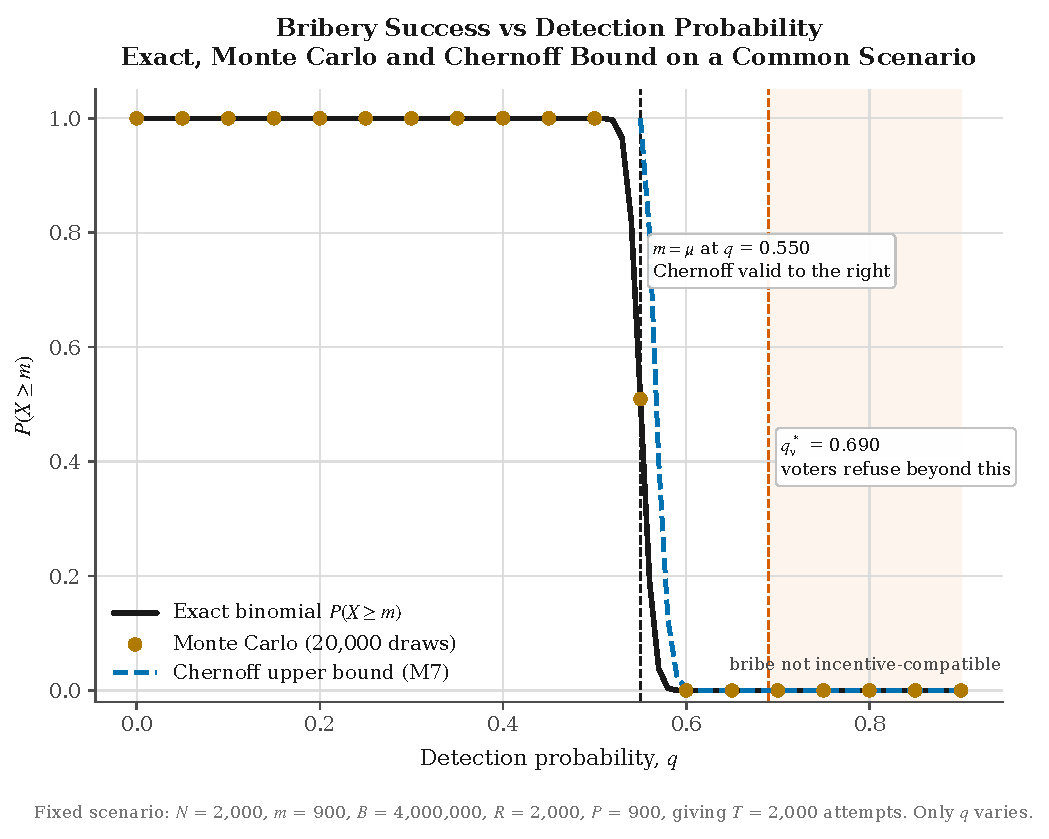
\includegraphics[width=0.97\textwidth]{fig_01_method_comparison.pdf}
\caption[Exact, Monte Carlo and Chernoff comparison]{Exact binomial,
Monte Carlo and Chernoff bound against detection probability on one
fixed scenario. Averaging these three quantities across heterogeneous
randomised trials would compare them on different sub-populations ---
the bound exists only where $m > \mu$ --- so this figure varies only
$q$.}
\label{fig:detection}
\end{figure}
\begin{readbox}\textsf{\bfseries How to read it.} Three independent methods on one scenario. The exact binomial curve and the Monte Carlo markers coincide throughout; the Chernoff curve sits above both wherever it is defined, which is the validity check. Where the bound disappears, $m \leq \mu$ and the one-sided upper tail does not apply. $R$ and $P$ are chosen so the collapse sits to the LEFT of $q_v^*$, i.e. inside the region where a rational voter would still accept the bribe.\end{readbox}
\clearpage
\begin{figure}[H]
\centering
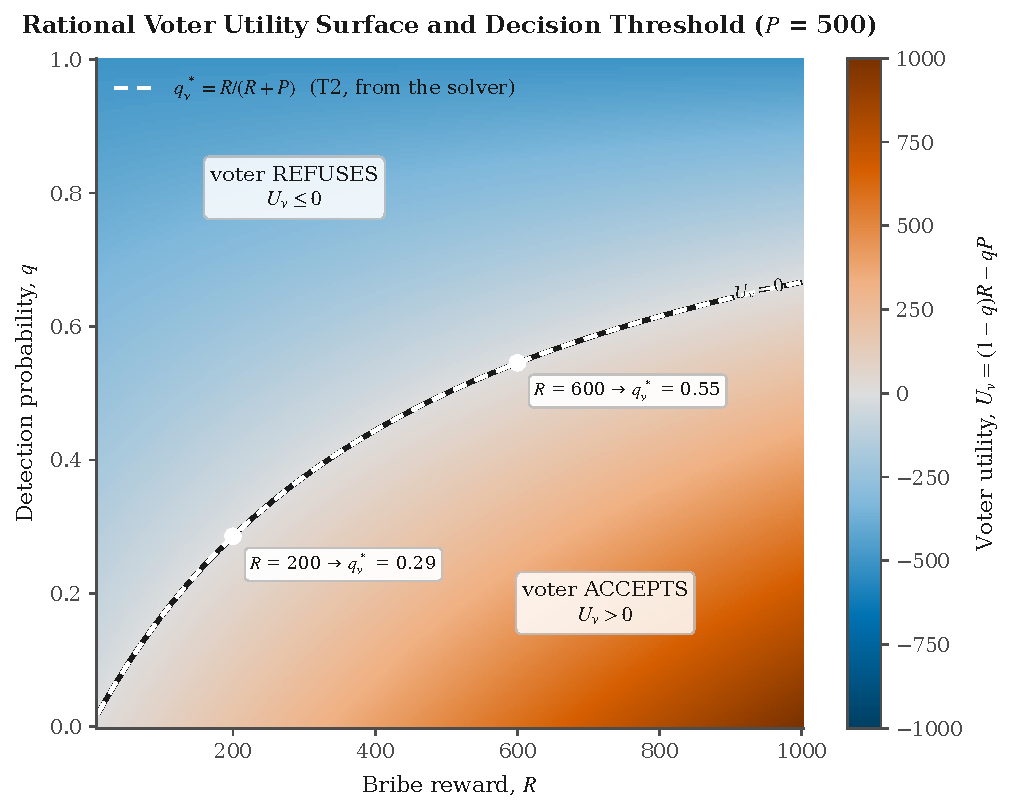
\includegraphics[width=0.97\textwidth]{fig_02_voter_utility_threshold.pdf}
\caption[Voter utility surface and decision threshold]{Rational voter
utility $\Uv = (1-q)R - qP$, with the $\Uv = 0$ decision boundary and
the closed-form indifference threshold $q_v^{*} = R/(R+P)$ drawn
together.}
\label{fig:utility}
\end{figure}
\begin{readbox}\textsf{\bfseries How to read it.} The rational-voter gate. A voter accepts a bribe only while $U_v = (1-q)R - qP$ stays positive; the crossing at $q_v^* = R/(R+P)$ is the point beyond which no budget buys a vote, because the voter --- not the system --- refuses.\end{readbox}
\clearpage
\begin{figure}[H]
\centering
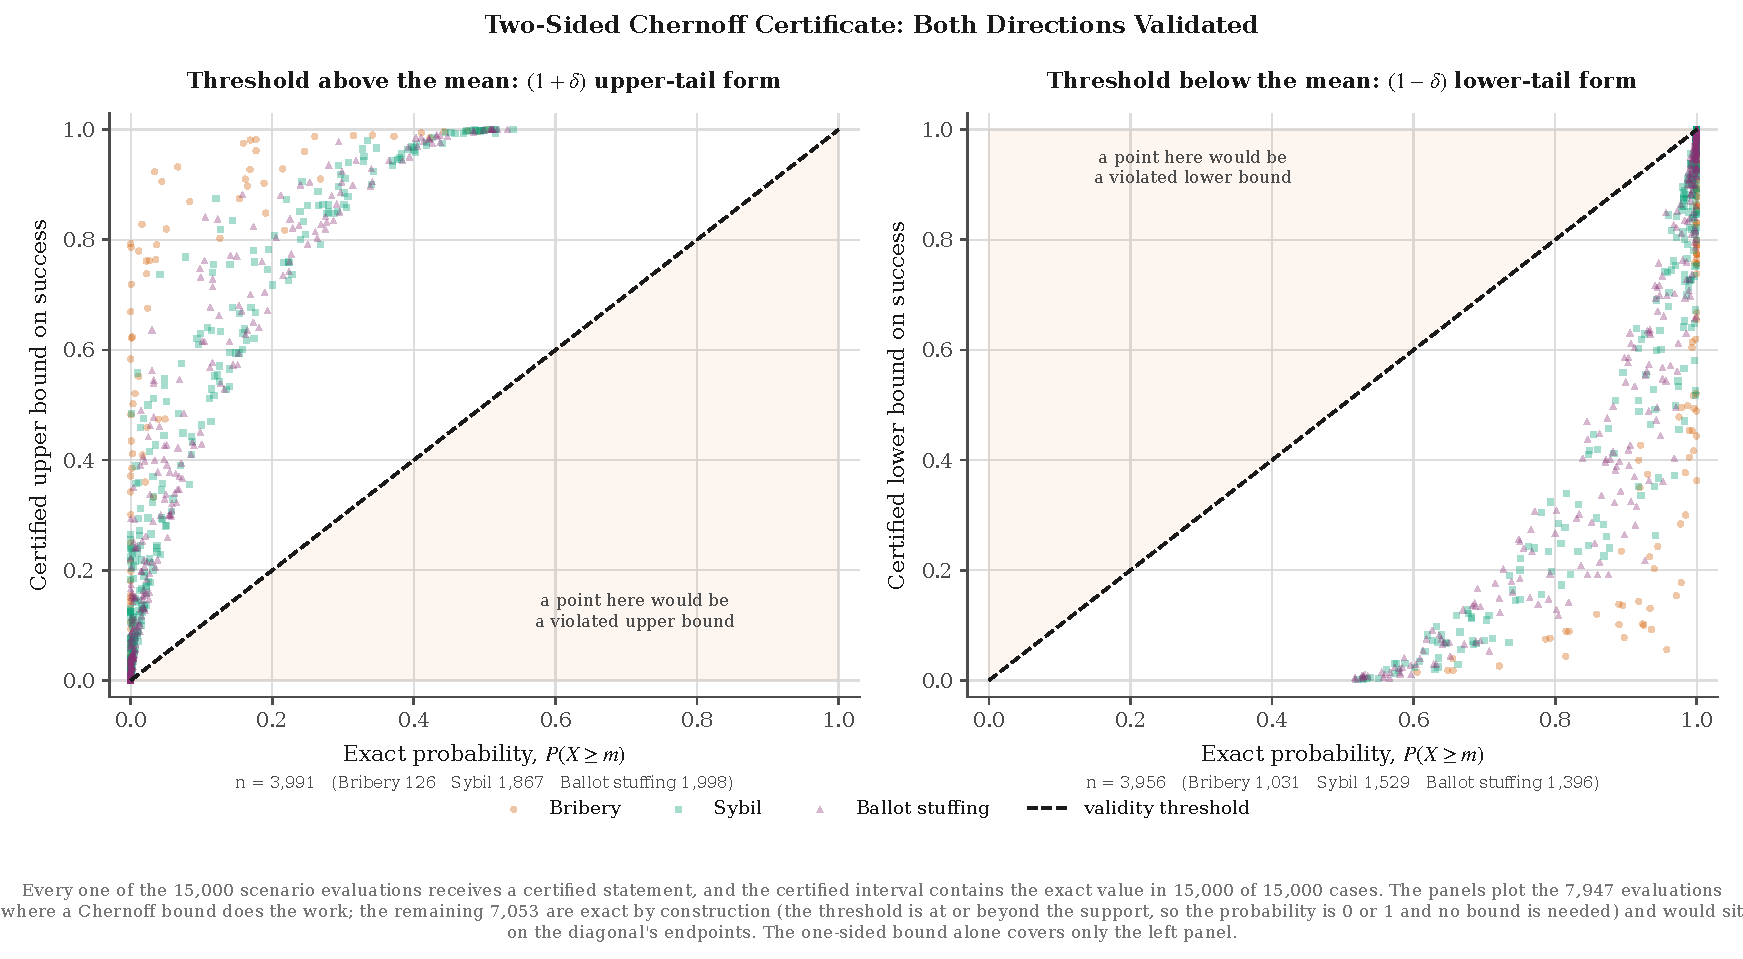
\includegraphics[width=\textwidth]{fig_03_chernoff_two_sided.pdf}
\caption[Two-sided Chernoff certificate]{Both Chernoff directions
validated. Left: threshold above the mean, where the $(1+\delta)$
upper-tail form certifies success from above --- valid points lie on or
above the diagonal. Right: threshold below the mean, where the
$(1-\delta)$ lower-tail form applied to the failure event certifies
success from below --- valid points lie on or below it. No point falls
on the wrong side of either diagonal.}
\label{fig:twosided}
\end{figure}
\begin{readbox}\textsf{\bfseries How to read it.} The two-sided Chernoff certificate. Every scenario now carries an analytic guarantee: an upper bound where $m > \mu$, and a lower bound obtained by applying the lower tail to the failure event where $m \leq \mu$. The exact value lies inside the certified interval in 100\% of evaluations.\end{readbox}
\clearpage
\begin{figure}[H]
\centering
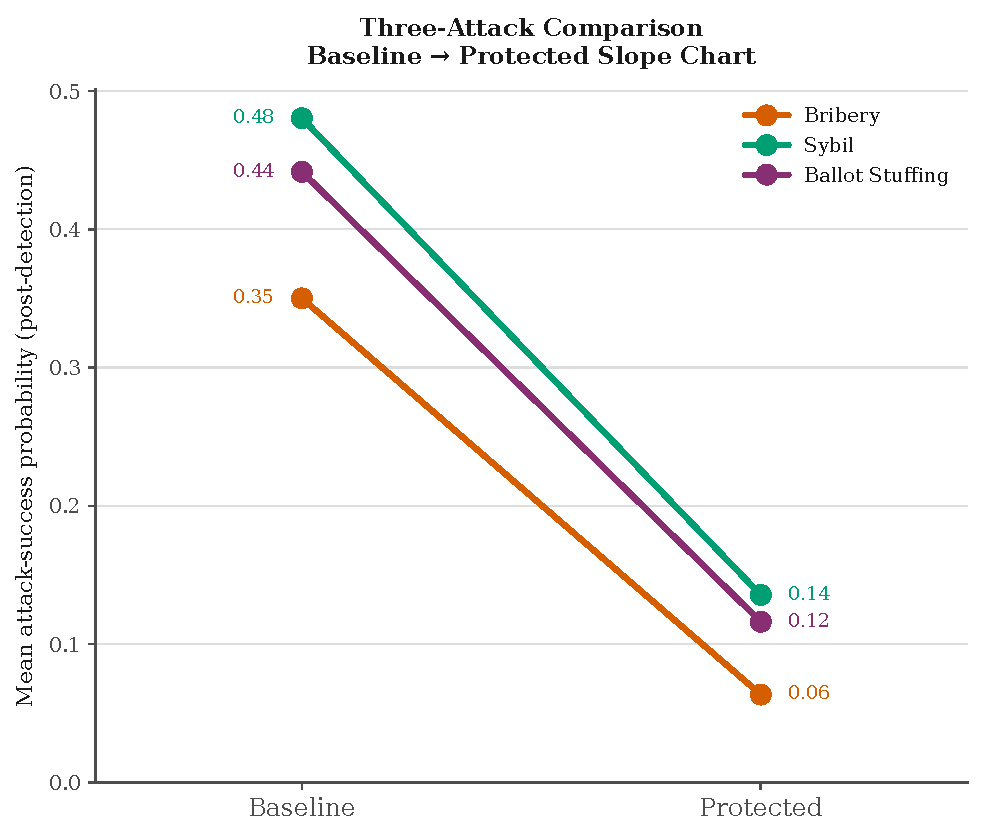
\includegraphics[width=0.97\textwidth]{fig_04_attack_comparison.pdf}
\caption[Three-attack comparison]{Mean success probability for the
three vectors, baseline against protected.}
\label{fig:comparison}
\end{figure}
\begin{readbox}\textsf{\bfseries How to read it.} The headline comparison. Baseline against protected, per vector, on identical paired trials. The gap between the two bars is the countermeasure effect; the error bars are bootstrap intervals, used because the underlying distributions are bimodal rather than normal. Note that the protected bars are reduced, not zero: attack success is substantially lowered under the modelled countermeasures, not eliminated.\end{readbox}
\clearpage
\begin{figure}[H]
\centering
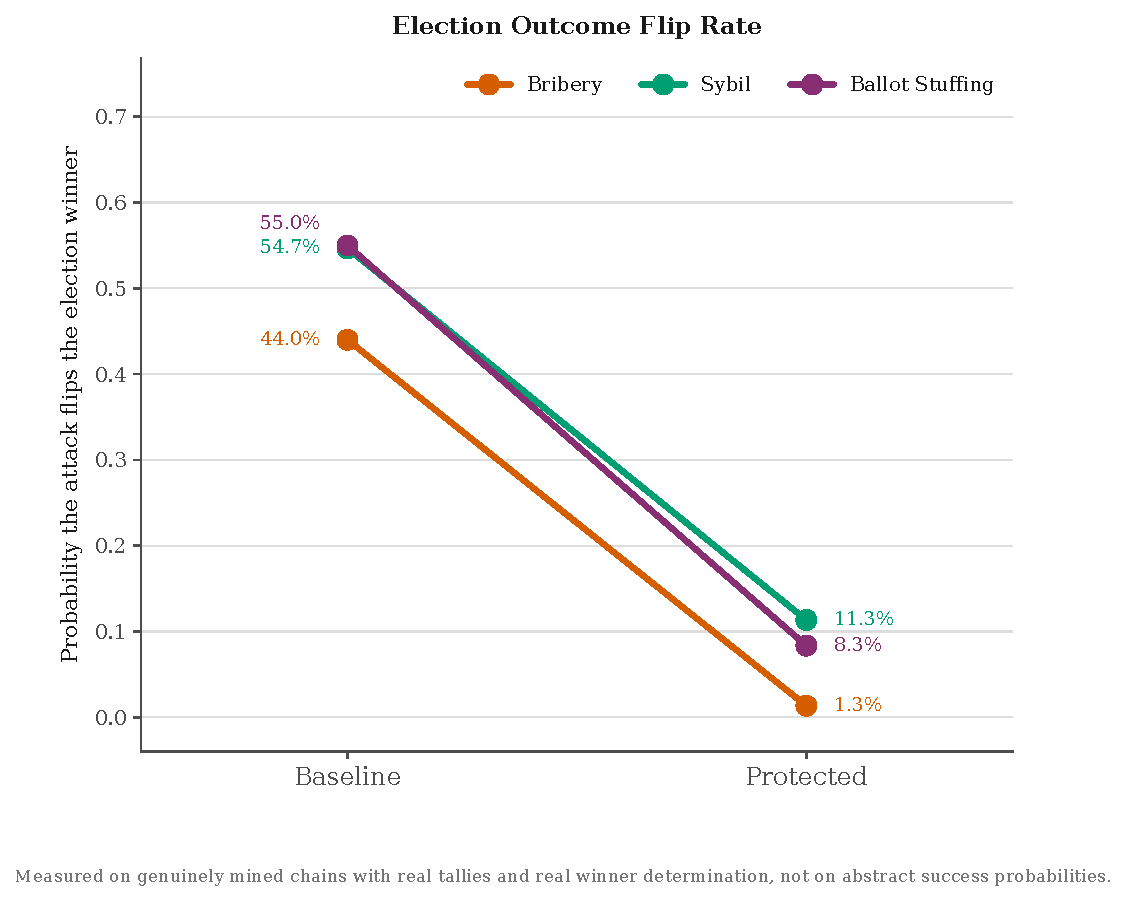
\includegraphics[width=0.97\textwidth]{fig_05_election_flip_rate.pdf}
\caption[Election outcome flip rate]{Probability that an attack flips
the winner of a concrete, blockchain-recorded election.}
\label{fig:flip}
\end{figure}
\begin{readbox}\textsf{\bfseries How to read it.} The concrete layer. Abstract success probability is one thing; the rate at which a mined election actually changes winner is another. This figure shows the two agree in magnitude, in the size of the protection effect, and in placing bribery lowest. They do not agree on the ordering of the top two: Sybil leads in the analytic layer and ballot stuffing here, by a third of a percentage point --- inside sampling error, so those two are best read as indistinguishable rather than ranked.\end{readbox}
\clearpage
\begin{figure}[H]
\centering
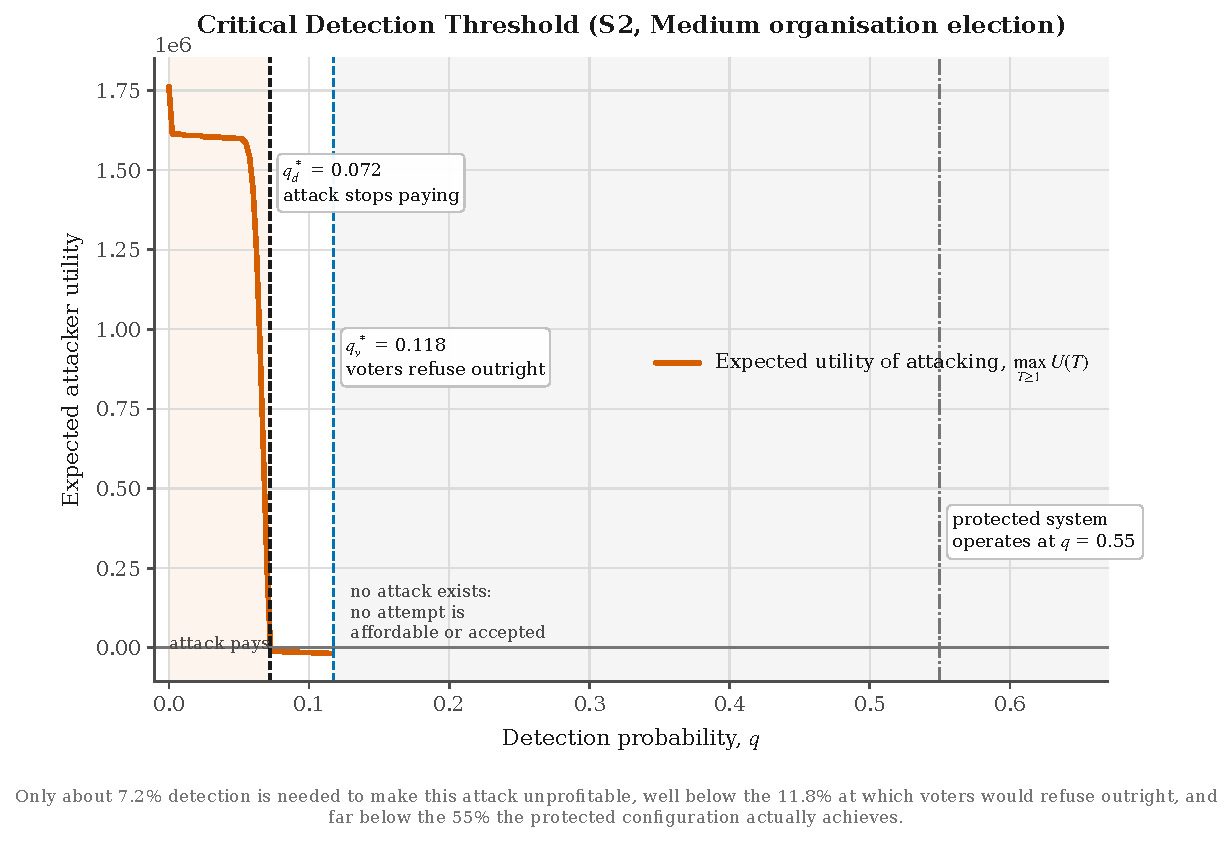
\includegraphics[width=0.97\textwidth]{fig_06_critical_detection.pdf}
\caption[Critical detection threshold]{Expected utility of attacking as
detection rises, for the medium-organisation scenario. Two thresholds
are marked: $q_d^{*}$, where the attack stops paying, and $q_v^{*}$,
where voters refuse outright.}
\label{fig:critical}
\end{figure}
\begin{readbox}\textsf{\bfseries How to read it.} The defender's design target. $q_d^*$ is where attacking stops paying --- the attacker still can, but no longer wants to. $q_v^*$ is where voters refuse outright. The gap between them is the region where deterrence relies on the attacker being rational. The protected configuration's much higher operating point is a deliberately generous margin in the model, not a level the analysis finds necessary --- far less detection would already deter.\end{readbox}
\clearpage
\begin{figure}[H]
\centering
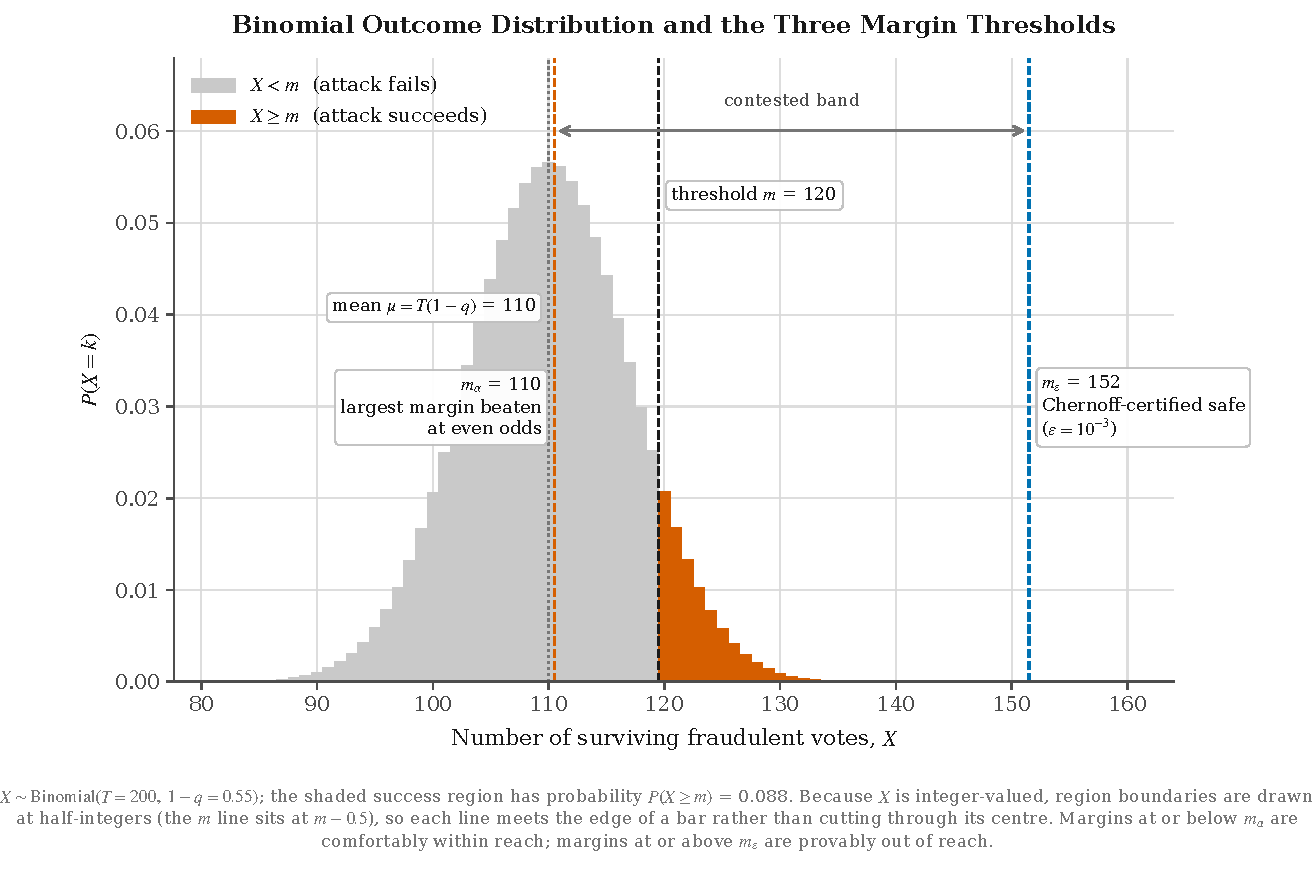
\includegraphics[width=0.97\textwidth]{fig_07_binomial_thresholds.pdf}
\caption[Binomial distribution with margin thresholds]{The binomial
outcome distribution with its mean, the manipulation threshold, the
attacker-reachable margin and the Chernoff-certified safe margin all
marked.}
\label{fig:pmf}
\end{figure}
\begin{readbox}\textsf{\bfseries How to read it.} The distribution behind every other figure, with all three margin thresholds drawn on it. Region boundaries sit at half-integers because $X$ is integer-valued, so each line meets the edge of a bar rather than cutting through its centre.\end{readbox}
\clearpage
\begin{figure}[H]
\centering
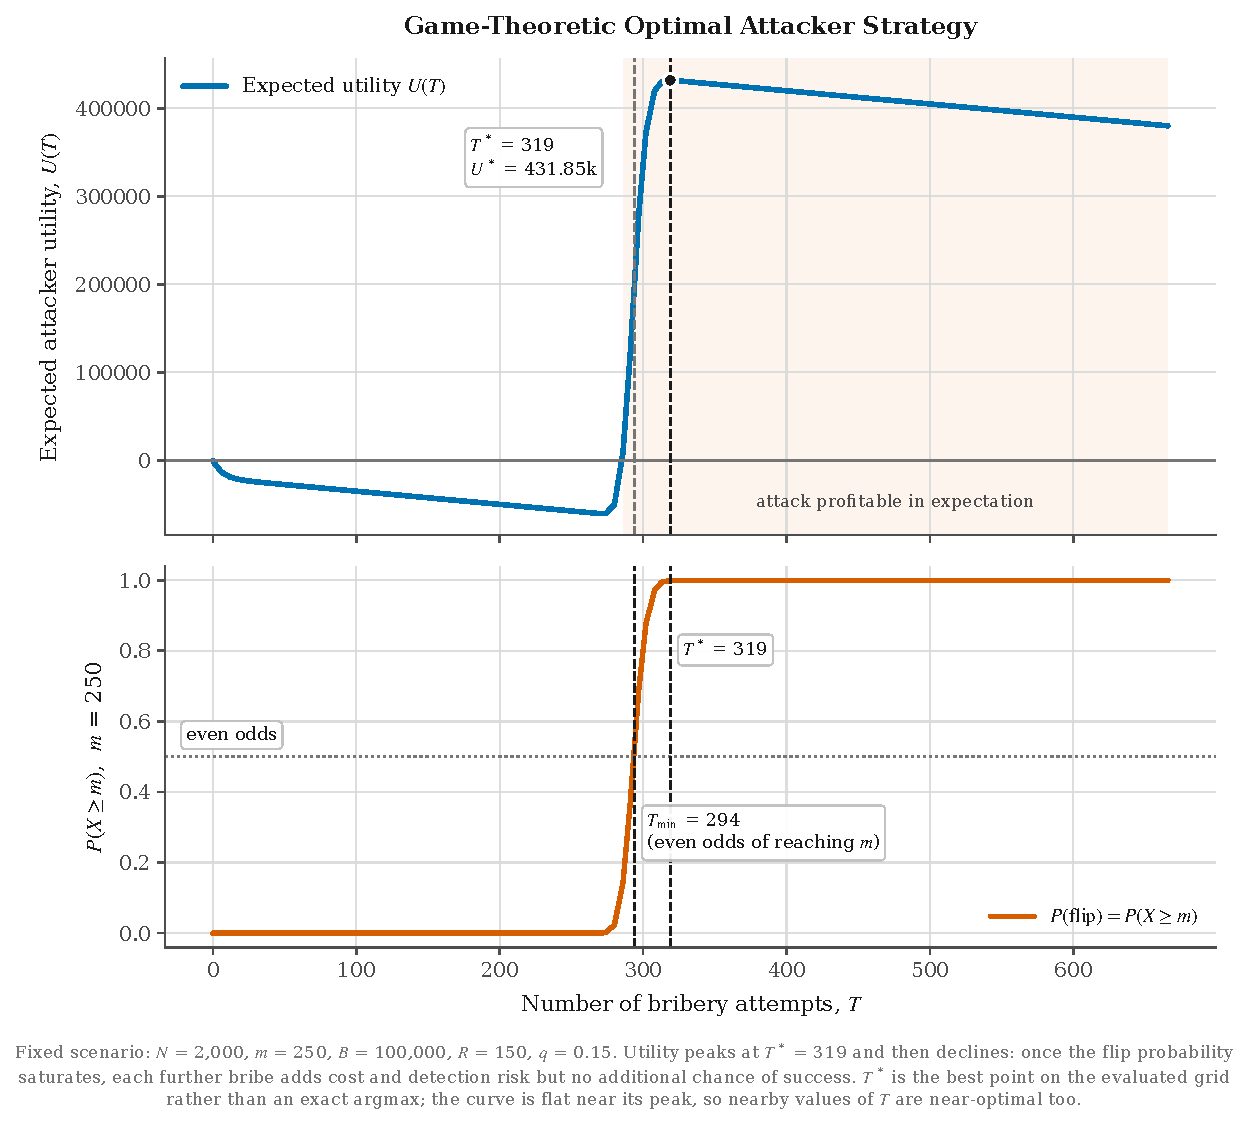
\includegraphics[width=0.97\textwidth]{fig_08_optimal_attacker.pdf}
\caption[Optimal attacker strategy]{Expected attacker utility (top) and
flip probability (bottom) against bribery attempts, with the
utility-maximising $T^{*}$ and the even-odds effort threshold
$T_{\min}$ marked.}
\label{fig:optimal}
\end{figure}
\begin{readbox}\textsf{\bfseries How to read it.} The attacker's optimisation. Utility against number of attempts, with the optimum marked. Effort beyond the optimum lowers utility, which is why a budget-constrained attacker does not simply spend everything.\end{readbox}
\clearpage
\begin{figure}[H]
\centering
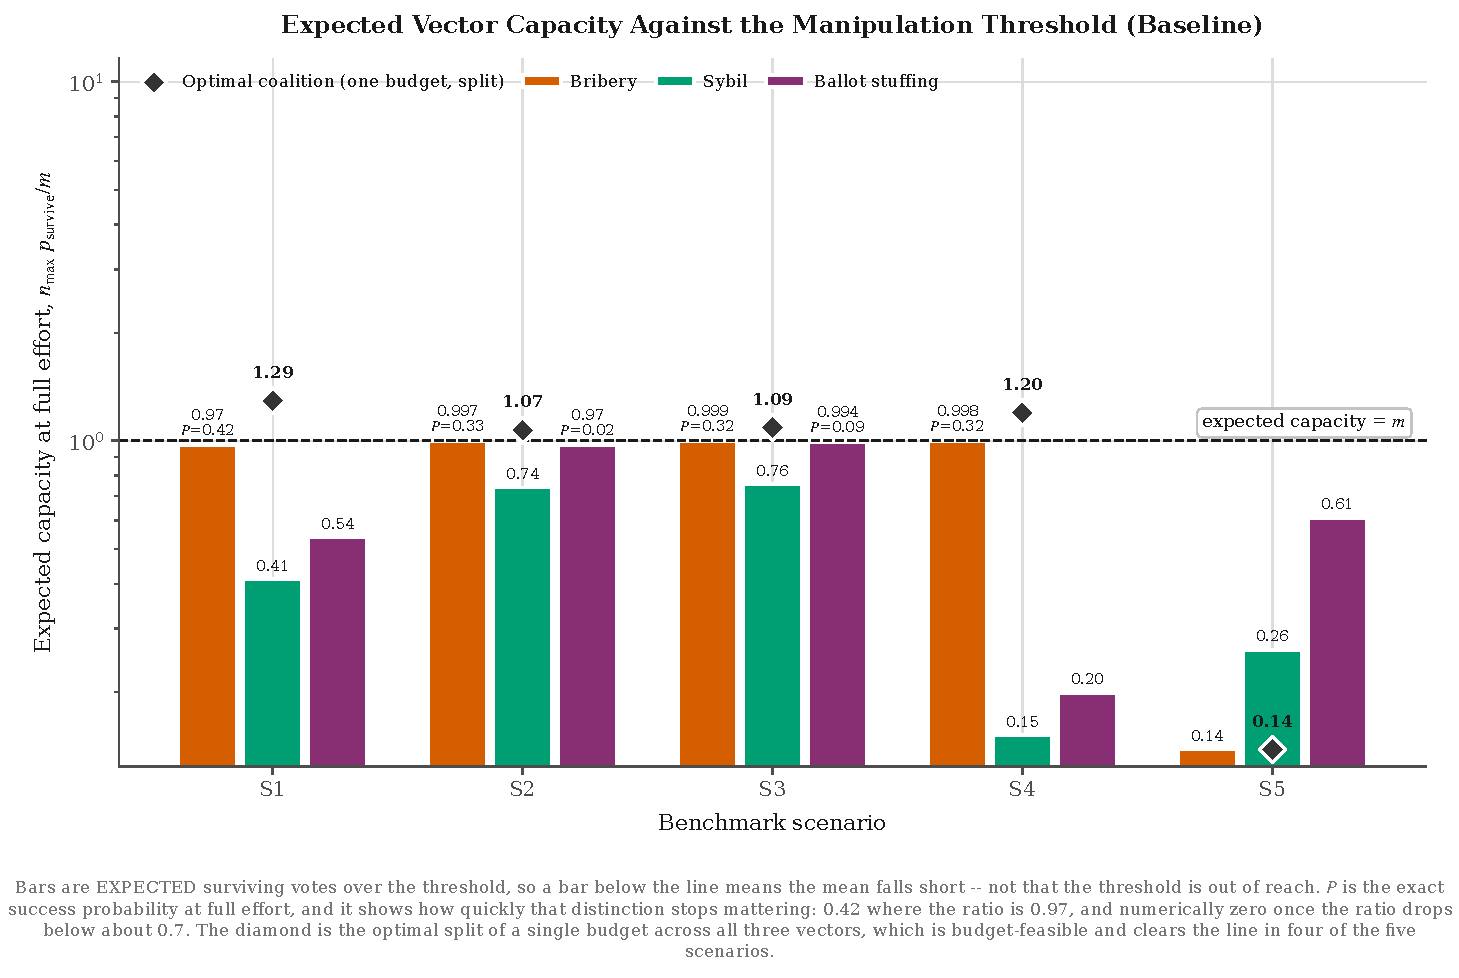
\includegraphics[width=0.97\textwidth]{fig_09_vector_capacity.pdf}
\caption[Vector capacity against the threshold]{\emph{Expected}
capacity of each vector at full effort, as a multiple of the
manipulation threshold. A bar below the line means the mean falls
short, not that the threshold is unreachable --- the annotated $P$ is
the exact success probability at full effort. The diamond is the
optimal split of a single budget across all three vectors, which is
budget-feasible.}
\label{fig:capacity}
\end{figure}
\begin{readbox}\textsf{\bfseries How to read it.} Why a rational attacker declines a vector. Each bar is capacity as a multiple of the threshold $m$, so the threshold is the line at 1.0. It is an EXPECTED value, not a ceiling: a bar below the line means the mean falls short, and the annotated $P$ gives the exact success probability at full effort --- 0.42 at a ratio of 0.97, and numerically zero below about 0.7. The diamond is the optimal split of one budget across all three vectors, which is budget-feasible.\end{readbox}
\clearpage
\begin{figure}[H]
\centering
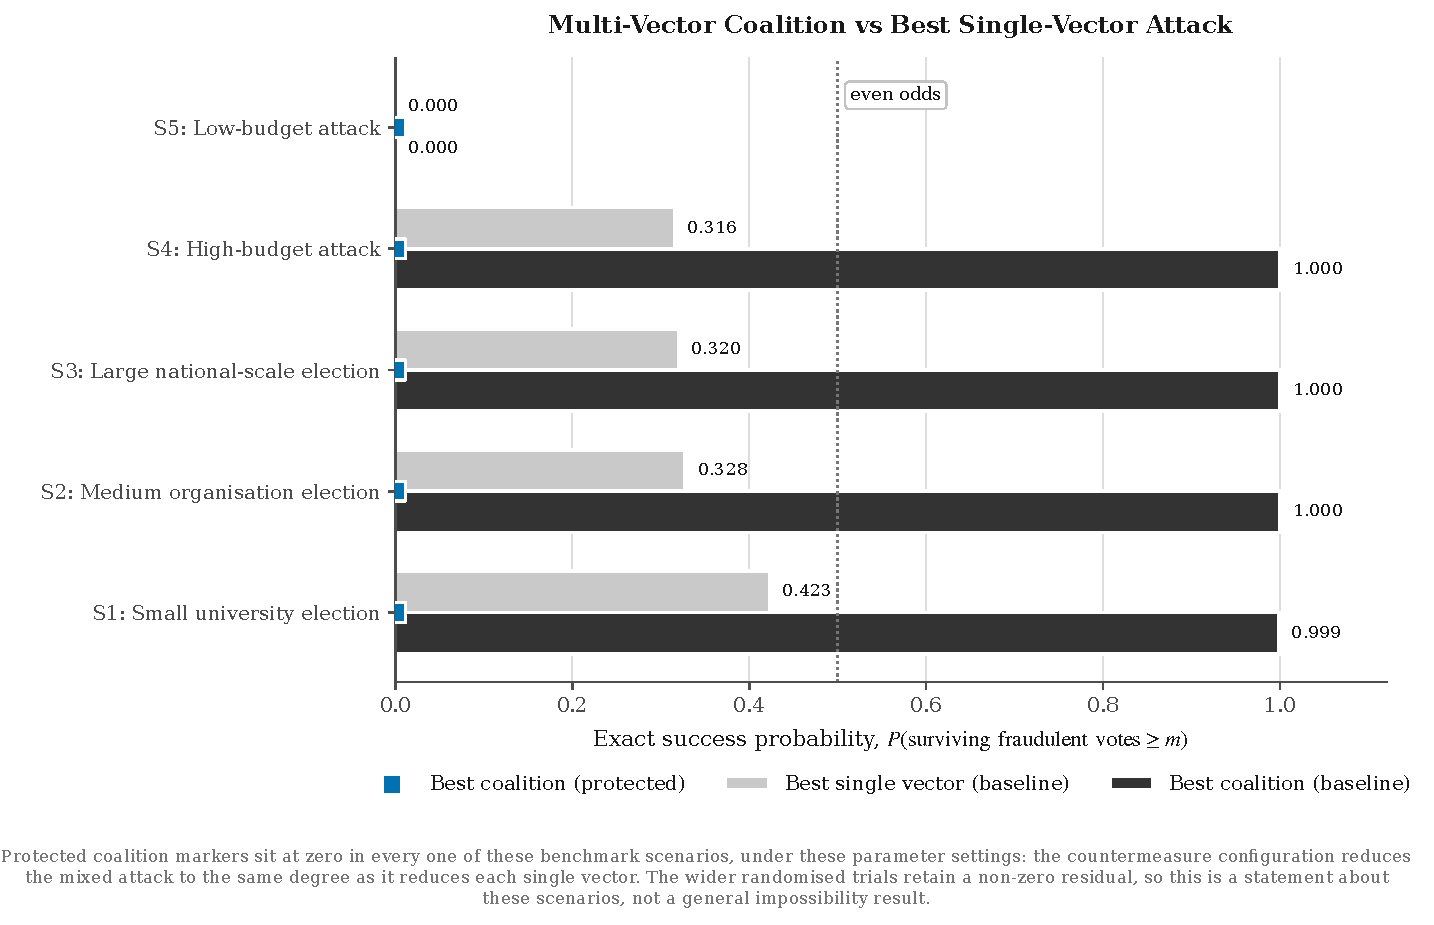
\includegraphics[width=0.97\textwidth]{fig_10_coalition_vs_pure.pdf}
\caption[Coalition against best single vector]{Best coalition attack
against best single-vector attack per scenario, with protected
coalition results overlaid.}
\label{fig:coalition}
\end{figure}
\begin{readbox}\textsf{\bfseries How to read it.} The coalition result. The best mixed-vector attack against the best single vector, per scenario. Protected markers sit at zero across these benchmark scenarios under these parameter settings --- a statement about those scenarios, not a general impossibility result, since the wider randomised trials retain a non-zero residual. Read the coalition analysis as an extension to the core baseline-versus-protected result, not as its centre.\end{readbox}
\clearpage

\section*{Part II. Result Tables}
\addcontentsline{toc}{section}{Part II. Result Tables}

The complete tabular output of the simulation, read directly from
\code{results/csv/}. Column names are as emitted by the pipeline.

\begin{readbox}
\textsf{\bfseries Which probability each table reports.} Sybil and ballot
stuffing pass fraudulent votes through \emph{two} independent gates, so they
have two success probabilities. $P(\text{accepted} \geq m)$ counts votes that
clear the \emph{acceptance} gate only --- an intermediate quantity that ignores
detection and is therefore always larger. $P(\text{surviving} \geq m)$ counts
votes that clear \emph{both} gates, and is the headline measure used in
Tables~7--9, Figure~4 and every stated conclusion. Bribery has one effective
gate (detection is folded into $1-q$), so its two measures coincide.
Tables~3 and~4 report both, labelled by a \code{measure} column; Tables~5 and
7--9 report the headline measure only, so the numbers agree across them.
\end{readbox}
\vspace{6pt}
\subsection*{Table 1. Parameter ranges used in the randomised trials}
\addcontentsline{toc}{subsection}{Table 1. Parameter ranges used in the randomised trials}
{\small
\setlength{\tabcolsep}{3pt}
\begin{longtable}{lll}
\toprule
parameter & low & high \\
\midrule
\endfirsthead
\toprule
parameter & low & high \\
\midrule
\endhead
\midrule
\multicolumn{3}{r}{Continued on next page} \\
\midrule
\endfoot
\bottomrule
\endlastfoot
N & 200.0000 & 5000.0000 \\
m\_fraction & 0.0200 & 0.2500 \\
B & 1000.0000 & 200000.0000 \\
R & 10.0000 & 500.0000 \\
P & 10.0000 & 2000.0000 \\
q\_baseline & 0.0200 & 0.2500 \\
q\_protected\_boost & 0.1500 & 0.6000 \\
S & 10.0000 & 1000.0000 \\
qs\_baseline & 0.4000 & 0.9500 \\
qs\_protected\_reduction & 0.3000 & 0.8000 \\
pd\_baseline & 0.0200 & 0.3000 \\
pd\_protected\_boost & 0.2000 & 0.7000 \\
A & 10.0000 & 1000.0000 \\
qb\_baseline & 0.3000 & 0.9000 \\
qb\_protected\_reduction & 0.3000 & 0.8000 \\
pb\_baseline & 0.0200 & 0.3000 \\
pb\_protected\_boost & 0.2000 & 0.7000 \\
\end{longtable}

}
\vspace{8pt}
\subsection*{Table 2. Bribery attack --- success probability (single gate: detection is folded into $1-q$)}
\addcontentsline{toc}{subsection}{Table 2. Bribery attack --- success probability (single gate: detection is folded into $1-q$)}
{\scriptsize
\setlength{\tabcolsep}{3pt}
\begin{longtable}{llllllll}
\toprule
attack & measure & system & mean & median & std & min & max \\
\midrule
\endfirsthead
\toprule
attack & measure & system & mean & median & std & min & max \\
\midrule
\endhead
\midrule
\multicolumn{8}{r}{Continued on next page} \\
\midrule
\endfoot
\bottomrule
\endlastfoot
bribery & single\_gate & baseline & 0.3501 & 0.0000 & 0.4743 & 0.0000 & 1.0000 \\
bribery & single\_gate & protected & 0.0635 & 0.0000 & 0.2421 & 0.0000 & 1.0000 \\
\end{longtable}

}
\vspace{8pt}
\subsection*{Table 3. Sybil attack --- both measures: surviving (headline) and accepted-only}
\addcontentsline{toc}{subsection}{Table 3. Sybil attack --- both measures: surviving (headline) and accepted-only}
{\scriptsize
\setlength{\tabcolsep}{3pt}
\begin{longtable}{llllllll}
\toprule
attack & measure & system & mean & median & std & min & max \\
\midrule
\endfirsthead
\toprule
attack & measure & system & mean & median & std & min & max \\
\midrule
\endhead
\midrule
\multicolumn{8}{r}{Continued on next page} \\
\midrule
\endfoot
\bottomrule
\endlastfoot
sybil & surviving\_ge\_m & baseline & 0.4804 & 0.0593 & 0.4923 & 0.0000 & 1.0000 \\
sybil & surviving\_ge\_m & protected & 0.1356 & 0.0000 & 0.3292 & 0.0000 & 1.0000 \\
sybil & accepted\_ge\_m & baseline & 0.5366 & 0.9993 & 0.4931 & 0.0000 & 1.0000 \\
sybil & accepted\_ge\_m & protected & 0.2991 & 0.0000 & 0.4486 & 0.0000 & 1.0000 \\
\end{longtable}

}
\vspace{8pt}
\subsection*{Table 4. Ballot stuffing --- both measures: surviving (headline) and accepted-only}
\addcontentsline{toc}{subsection}{Table 4. Ballot stuffing --- both measures: surviving (headline) and accepted-only}
{\scriptsize
\setlength{\tabcolsep}{3pt}
\begin{longtable}{llllllll}
\toprule
attack & measure & system & mean & median & std & min & max \\
\midrule
\endfirsthead
\toprule
attack & measure & system & mean & median & std & min & max \\
\midrule
\endhead
\midrule
\multicolumn{8}{r}{Continued on next page} \\
\midrule
\endfoot
\bottomrule
\endlastfoot
ballot\_stuffing & surviving\_ge\_m & baseline & 0.4416 & 0.0000 & 0.4871 & 0.0000 & 1.0000 \\
ballot\_stuffing & surviving\_ge\_m & protected & 0.1162 & 0.0000 & 0.3098 & 0.0000 & 1.0000 \\
ballot\_stuffing & accepted\_ge\_m & baseline & 0.4979 & 0.4834 & 0.4926 & 0.0000 & 1.0000 \\
ballot\_stuffing & accepted\_ge\_m & protected & 0.2535 & 0.0000 & 0.4239 & 0.0000 & 1.0000 \\
\end{longtable}

}
\vspace{8pt}
\subsection*{Table 5. Baseline versus protected --- headline measure only (agrees with Tables 7--9)}
\addcontentsline{toc}{subsection}{Table 5. Baseline versus protected --- headline measure only (agrees with Tables 7--9)}
{\scriptsize
\setlength{\tabcolsep}{3pt}
\begin{longtable}{llllllll}
\toprule
attack & measure & system & mean & median & std & min & max \\
\midrule
\endfirsthead
\toprule
attack & measure & system & mean & median & std & min & max \\
\midrule
\endhead
\midrule
\multicolumn{8}{r}{Continued on next page} \\
\midrule
\endfoot
\bottomrule
\endlastfoot
bribery & single\_gate & baseline & 0.3501 & 0.0000 & 0.4743 & 0.0000 & 1.0000 \\
bribery & single\_gate & protected & 0.0635 & 0.0000 & 0.2421 & 0.0000 & 1.0000 \\
sybil & surviving\_ge\_m & baseline & 0.4804 & 0.0593 & 0.4923 & 0.0000 & 1.0000 \\
sybil & surviving\_ge\_m & protected & 0.1356 & 0.0000 & 0.3292 & 0.0000 & 1.0000 \\
ballot\_stuffing & surviving\_ge\_m & baseline & 0.4416 & 0.0000 & 0.4871 & 0.0000 & 1.0000 \\
ballot\_stuffing & surviving\_ge\_m & protected & 0.1162 & 0.0000 & 0.3098 & 0.0000 & 1.0000 \\
\end{longtable}

}
\vspace{8pt}
\subsection*{Table 6. Chernoff bound validation statistics}
\addcontentsline{toc}{subsection}{Table 6. Chernoff bound validation statistics}
{\scriptsize
\setlength{\tabcolsep}{3pt}
\begin{longtable}{llllll}
\toprule
n valid & mean conservativeness & min conservativeness & max conservativeness & pct bound holds & attack \\
\midrule
\endfirsthead
\toprule
n valid & mean conservativeness & min conservativeness & max conservativeness & pct bound holds & attack \\
\midrule
\endhead
\midrule
\multicolumn{6}{r}{Continued on next page} \\
\midrule
\endfoot
\bottomrule
\endlastfoot
1088 & 0.0423 & 0.0000 & 0.8896 & 100.0000 & bribery \\
3471 & 0.0260 & 0.0000 & 0.7550 & 100.0000 & sybil \\
3604 & 0.0216 & 0.0000 & 0.7360 & 100.0000 & ballot\_stuffing \\
\end{longtable}

}
\vspace{8pt}
\begin{landscape}
\subsection*{Table 7. Statistical analysis of the paired design}
\addcontentsline{toc}{subsection}{Table 7. Statistical analysis of the paired design}
{\tiny
\setlength{\tabcolsep}{3pt}
\begin{longtable}{llllllllll}
\toprule
mean baseline & mean protected & absolute reduction & relative reduction & mean paired reduction & paired reduction std & bootstrap boot mean & bootstrap ci low & bootstrap ci high & attack type \\
\midrule
\endfirsthead
\toprule
mean baseline & mean protected & absolute reduction & relative reduction & mean paired reduction & paired reduction std & bootstrap boot mean & bootstrap ci low & bootstrap ci high & attack type \\
\midrule
\endhead
\midrule
\multicolumn{10}{r}{Continued on next page} \\
\midrule
\endfoot
\bottomrule
\endlastfoot
0.3501 & 0.0635 & 0.2866 & 0.8186 & 0.2866 & 0.4483 & 0.2864 & 0.2689 & 0.3041 & bribery \\
0.4804 & 0.1356 & 0.3448 & 0.7178 & 0.3448 & 0.4580 & 0.3445 & 0.3268 & 0.3622 & sybil \\
0.4416 & 0.1162 & 0.3255 & 0.7370 & 0.3255 & 0.4510 & 0.3256 & 0.3084 & 0.3432 & ballot\_stuffing \\
\end{longtable}

}
\end{landscape}
\subsection*{Table 8. Countermeasure effectiveness (absolute and relative reduction)}
\addcontentsline{toc}{subsection}{Table 8. Countermeasure effectiveness (absolute and relative reduction)}
{\small
\setlength{\tabcolsep}{3pt}
\begin{longtable}{lllll}
\toprule
attack type & mean baseline & mean protected & absolute reduction & relative reduction \\
\midrule
\endfirsthead
\toprule
attack type & mean baseline & mean protected & absolute reduction & relative reduction \\
\midrule
\endhead
\midrule
\multicolumn{5}{r}{Continued on next page} \\
\midrule
\endfoot
\bottomrule
\endlastfoot
bribery & 0.3501 & 0.0635 & 0.2866 & 0.8186 \\
sybil & 0.4804 & 0.1356 & 0.3448 & 0.7178 \\
ballot\_stuffing & 0.4416 & 0.1162 & 0.3255 & 0.7370 \\
\end{longtable}

}
\vspace{8pt}
\subsection*{Table 9. Overall attack comparison across the three vectors}
\addcontentsline{toc}{subsection}{Table 9. Overall attack comparison across the three vectors}
{\scriptsize
\setlength{\tabcolsep}{3pt}
\begin{longtable}{llllll}
\toprule
attack & mean baseline success & mean protected success & relative reduction pct & mc mean abs error & chernoff pct holds \\
\midrule
\endfirsthead
\toprule
attack & mean baseline success & mean protected success & relative reduction pct & mc mean abs error & chernoff pct holds \\
\midrule
\endhead
\midrule
\multicolumn{6}{r}{Continued on next page} \\
\midrule
\endfoot
\bottomrule
\endlastfoot
bribery & 0.3501 & 0.0635 & 81.8589 & 0.0001 & 100.0000 \\
sybil & 0.4804 & 0.1356 & 71.7790 & 0.0004 & 100.0000 \\
ballot\_stuffing & 0.4416 & 0.1162 & 73.6953 & 0.0004 & 100.0000 \\
\end{longtable}

}
\vspace{8pt}
\begin{landscape}
\subsection*{Table 10. Sample scenarios with the manipulation threshold $m$}
\addcontentsline{toc}{subsection}{Table 10. Sample scenarios with the manipulation threshold $m$}
{\tiny
\setlength{\tabcolsep}{3pt}
\begin{longtable}{llllllllll}
\toprule
trial id & N & m & B & R & P & q & system type & exact probability & attack success exact \\
\midrule
\endfirsthead
\toprule
trial id & N & m & B & R & P & q & system type & exact probability & attack success exact \\
\midrule
\endhead
\midrule
\multicolumn{10}{r}{Continued on next page} \\
\midrule
\endfoot
\bottomrule
\endlastfoot
1 & 2266 & 275 & 122751.5049 & 257.4784 & 1479.1157 & 0.0842 & baseline & 1.0000 & True \\
1 & 2266 & 275 & 122751.5049 & 257.4784 & 1479.1157 & 0.2615 & protected & 0.0000 & False \\
2 & 4853 & 600 & 122396.0345 & 457.0915 & 1175.7973 & 0.1742 & baseline & 0.0000 & False \\
2 & 4853 & 600 & 122396.0345 & 457.0915 & 1175.7973 & 0.6655 & protected & 0.0000 & False \\
3 & 2832 & 325 & 48399.9988 & 339.8336 & 617.3681 & 0.1135 & baseline & 0.0000 & False \\
3 & 2832 & 325 & 48399.9988 & 339.8336 & 617.3681 & 0.3816 & protected & 0.0000 & False \\
4 & 2185 & 170 & 54426.8507 & 80.3503 & 1612.2060 & 0.0301 & baseline & 1.0000 & True \\
4 & 2185 & 170 & 54426.8507 & 80.3503 & 1612.2060 & 0.2908 & protected & 0.0000 & False \\
5 & 1339 & 28 & 32524.0897 & 268.5447 & 987.8435 & 0.1716 & baseline & 1.0000 & True \\
5 & 1339 & 28 & 32524.0897 & 268.5447 & 987.8435 & 0.4312 & protected & 0.0000 & False \\
6 & 4602 & 366 & 93406.3314 & 261.9435 & 1659.2226 & 0.2452 & baseline & 0.0000 & False \\
6 & 4602 & 366 & 93406.3314 & 261.9435 & 1659.2226 & 0.3740 & protected & 0.0000 & False \\
7 & 1215 & 176 & 53865.9070 & 342.5107 & 1767.2102 & 0.1220 & baseline & 0.0000 & False \\
7 & 1215 & 176 & 53865.9070 & 342.5107 & 1767.2102 & 0.5104 & protected & 0.0000 & False \\
8 & 301 & 42 & 16428.4483 & 497.2649 & 1961.4240 & 0.0719 & baseline & 0.0000 & False \\
8 & 301 & 42 & 16428.4483 & 497.2649 & 1961.4240 & 0.2514 & protected & 0.0000 & False \\
9 & 945 & 197 & 171607.6095 & 200.9098 & 417.8600 & 0.0833 & baseline & 1.0000 & True \\
9 & 945 & 197 & 171607.6095 & 200.9098 & 417.8600 & 0.3743 & protected & 0.0000 & False \\
10 & 3174 & 308 & 18530.7135 & 403.8856 & 1403.6775 & 0.2330 & baseline & 0.0000 & False \\
10 & 3174 & 308 & 18530.7135 & 403.8856 & 1403.6775 & 0.3850 & protected & 0.0000 & False \\
11 & 3779 & 710 & 98080.1864 & 64.3038 & 1942.2510 & 0.0745 & baseline & 0.0000 & False \\
11 & 3779 & 710 & 98080.1864 & 64.3038 & 1942.2510 & 0.2938 & protected & 0.0000 & False \\
12 & 4311 & 956 & 37465.0252 & 82.2381 & 131.7993 & 0.1598 & baseline & 0.0000 & False \\
12 & 4311 & 956 & 37465.0252 & 82.2381 & 131.7993 & 0.5154 & protected & 0.0000 & False \\
13 & 1855 & 287 & 181786.9165 & 89.5474 & 862.7410 & 0.1241 & baseline & 0.0000 & False \\
13 & 1855 & 287 & 181786.9165 & 89.5474 & 862.7410 & 0.3897 & protected & 0.0000 & False \\
14 & 3885 & 393 & 25016.9646 & 154.7345 & 476.1860 & 0.2479 & baseline & 0.0000 & False \\
14 & 3885 & 393 & 25016.9646 & 154.7345 & 476.1860 & 0.4073 & protected & 0.0000 & False \\
15 & 4092 & 973 & 55194.9407 & 206.1441 & 1075.9624 & 0.1898 & baseline & 0.0000 & False \\
15 & 4092 & 973 & 55194.9407 & 206.1441 & 1075.9624 & 0.3552 & protected & 0.0000 & False \\
\end{longtable}

}
\end{landscape}
\begin{landscape}
\subsection*{Table 11. Critical thresholds T1--T7 per benchmark scenario}
\addcontentsline{toc}{subsection}{Table 11. Critical thresholds T1--T7 per benchmark scenario}
{\tiny
\setlength{\tabcolsep}{3pt}
\resizebox{\linewidth}{!}{%
\begin{tabular}{llllllllllllllllllllll}
\toprule
scenario id & name & system type & N & m & B & R & P & q & R star & q voter indifference & voter accepts & T feasible & T star & T min for even odds & B star & q defender critical & mu & m reachable & m certified & exact p flip & utility star \\
\midrule
S1 & Small university election (100 voters) & baseline & 100 & 35 & 3000 & 80 & 600 & 0.0800 & 52.1739 & 0.1176 & True & 37 & 37 & 38.0000 & 2880.0000 & 0.1176 & 34.0400 & 34.0000 & NaN & 0.4231 & 21471.9356 \\
S1 & Small university election (100 voters) & protected & 100 & 35 & 3000 & 80 & 600 & 0.5500 & 733.3333 & 0.1176 & False & 37 & 0 & 77.0000 & NaN & 0.1176 & 16.6500 & 17.0000 & 34.0000 & 0.0000 & 0.0000 \\
S2 & Medium organisation election (10,000 voters) & baseline & 10000 & 1943 & 250000 & 120 & 900 & 0.0700 & 67.7419 & 0.1176 & True & 2083 & 2083 & 2089.0000 & 249480.0002 & 0.0722 & 1937.1900 & 1937.0000 & NaN & 0.3277 & 255503.1621 \\
S2 & Medium organisation election (10,000 voters) & protected & 10000 & 1943 & 250000 & 120 & 900 & 0.5500 & 1100.0000 & 0.1176 & False & 2083 & 0 & 4317.0000 & NaN & 0.0722 & 937.3500 & 937.0000 & 1054.0000 & 0.0000 & 0.0000 \\
S3 & Large national-scale election (100,000 voters) & baseline & 100000 & 19015 & 3000000 & 150 & 1200 & 0.0500 & 63.1579 & 0.1111 & True & 20000 & 20000 & 20016.0000 & 2998649.9998 & 0.0504 & 19000.0000 & 19000.0000 & 19515.0000 & 0.3204 & 1907536.0062 \\
S3 & Large national-scale election (100,000 voters) & protected & 100000 & 19015 & 3000000 & 150 & 1200 & 0.5500 & 1466.6667 & 0.1111 & False & 20000 & 0 & 42255.0000 & NaN & 0.0504 & 9000.0000 & 9000.0000 & NaN & 0.0000 & 0.0000 \\
S4 & High-budget attack (maximum attacker capability) & baseline & 5000 & 4758 & 5000000 & 100 & 500 & 0.0500 & 26.3158 & 0.1667 & True & 5000 & 5000 & 5008.0000 & 499400.0004 & 0.0514 & 4750.0000 & 4750.0000 & NaN & 0.3159 & 679480.1805 \\
S4 & High-budget attack (maximum attacker capability) & protected & 5000 & 4758 & 5000000 & 100 & 500 & 0.5500 & 611.1111 & 0.1667 & False & 5000 & 0 & 10573.0000 & NaN & 0.0514 & 2250.0000 & 2250.0000 & NaN & 0.0000 & 0.0000 \\
S5 & Low-budget attack (expected to fail) & baseline & 5000 & 550 & 8000 & 100 & 500 & 0.0500 & 26.3158 & 0.1667 & True & 80 & 0 & 579.0000 & 57100.0004 & 0.0000 & 76.0000 & 76.0000 & NaN & 0.0000 & 0.0000 \\
S5 & Low-budget attack (expected to fail) & protected & 5000 & 550 & 8000 & 100 & 500 & 0.5500 & 611.1111 & 0.1667 & False & 80 & 0 & 1222.0000 & NaN & 0.0000 & 36.0000 & 36.0000 & 61.0000 & 0.0000 & 0.0000 \\
\bottomrule
\end{tabular}
}
}
\end{landscape}
\begin{landscape}
\subsection*{Table 12. Optimal attacker effort per vector (G1)}
\addcontentsline{toc}{subsection}{Table 12. Optimal attacker effort per vector (G1)}
{\tiny
\setlength{\tabcolsep}{3pt}
\resizebox{\linewidth}{!}{%
\begin{tabular}{lllllllllllllll}
\toprule
scenario id & name & system type & vector & unit cost & p survive & p detect & m & n feasible & n star & p success at star & cost at star & utility star & viable & gate open \\
\midrule
S1 & Small university election (100 voters) & baseline & bribery & 80.0000 & 0.9200 & 0.0800 & 35 & 37 & 37 & 0.4231 & 2960.0000 & 21471.9356 & True & True \\
S1 & Small university election (100 voters) & baseline & sybil & 32.0000 & 0.7200 & 0.1000 & 35 & 20 & 0 & 0.0000 & 0.0000 & 0.0000 & False & True \\
S1 & Small university election (100 voters) & baseline & ballot\_stuffing & 12.0000 & 0.6300 & 0.1000 & 35 & 30 & 0 & 0.0000 & 0.0000 & 0.0000 & False & True \\
S1 & Small university election (100 voters) & protected & bribery & 80.0000 & 0.4500 & 0.5500 & 35 & 37 & 0 & 0.0000 & 0.0000 & 0.0000 & False & False \\
S1 & Small university election (100 voters) & protected & sybil & 32.0000 & 0.1125 & 0.5500 & 35 & 20 & 0 & 0.0000 & 0.0000 & 0.0000 & False & True \\
S1 & Small university election (100 voters) & protected & ballot\_stuffing & 12.0000 & 0.0900 & 0.5500 & 35 & 30 & 0 & 0.0000 & 0.0000 & 0.0000 & False & True \\
S2 & Medium organisation election (10,000 voters) & baseline & bribery & 120.0000 & 0.9300 & 0.0700 & 1943 & 2083 & 2083 & 0.3277 & 249960.0000 & 255503.1621 & True & True \\
S2 & Medium organisation election (10,000 voters) & baseline & sybil & 48.0000 & 0.7200 & 0.1000 & 1943 & 2000 & 0 & 0.0000 & 0.0000 & 0.0000 & False & True \\
S2 & Medium organisation election (10,000 voters) & baseline & ballot\_stuffing & 18.0000 & 0.6300 & 0.1000 & 1943 & 3000 & 0 & 0.0000 & 0.0000 & 0.0000 & False & True \\
S2 & Medium organisation election (10,000 voters) & protected & bribery & 120.0000 & 0.4500 & 0.5500 & 1943 & 2083 & 0 & 0.0000 & 0.0000 & 0.0000 & False & False \\
S2 & Medium organisation election (10,000 voters) & protected & sybil & 48.0000 & 0.1125 & 0.5500 & 1943 & 2000 & 0 & 0.0000 & 0.0000 & 0.0000 & False & True \\
S2 & Medium organisation election (10,000 voters) & protected & ballot\_stuffing & 18.0000 & 0.0900 & 0.5500 & 1943 & 3000 & 0 & 0.0000 & 0.0000 & 0.0000 & False & True \\
S3 & Large national-scale election (100,000 voters) & baseline & bribery & 150.0000 & 0.9500 & 0.0500 & 19015 & 20000 & 20000 & 0.3204 & 3000000.0000 & 1907536.0062 & True & True \\
S3 & Large national-scale election (100,000 voters) & baseline & sybil & 60.0000 & 0.7200 & 0.1000 & 19015 & 20000 & 0 & 0.0000 & 0.0000 & 0.0000 & False & True \\
S3 & Large national-scale election (100,000 voters) & baseline & ballot\_stuffing & 22.5000 & 0.6300 & 0.1000 & 19015 & 30000 & 0 & 0.0000 & 0.0000 & 0.0000 & False & True \\
S3 & Large national-scale election (100,000 voters) & protected & bribery & 150.0000 & 0.4500 & 0.5500 & 19015 & 20000 & 0 & 0.0000 & 0.0000 & 0.0000 & False & False \\
S3 & Large national-scale election (100,000 voters) & protected & sybil & 60.0000 & 0.1125 & 0.5500 & 19015 & 20000 & 0 & 0.0000 & 0.0000 & 0.0000 & False & True \\
S3 & Large national-scale election (100,000 voters) & protected & ballot\_stuffing & 22.5000 & 0.0900 & 0.5500 & 19015 & 30000 & 0 & 0.0000 & 0.0000 & 0.0000 & False & True \\
S4 & High-budget attack (maximum attacker capability) & baseline & bribery & 100.0000 & 0.9500 & 0.0500 & 4758 & 5000 & 5000 & 0.3159 & 500000.0000 & 679480.1805 & True & True \\
S4 & High-budget attack (maximum attacker capability) & baseline & sybil & 40.0000 & 0.7200 & 0.1000 & 4758 & 1000 & 0 & 0.0000 & 0.0000 & 0.0000 & False & True \\
S4 & High-budget attack (maximum attacker capability) & baseline & ballot\_stuffing & 15.0000 & 0.6300 & 0.1000 & 4758 & 1500 & 0 & 0.0000 & 0.0000 & 0.0000 & False & True \\
S4 & High-budget attack (maximum attacker capability) & protected & bribery & 100.0000 & 0.4500 & 0.5500 & 4758 & 5000 & 0 & 0.0000 & 0.0000 & 0.0000 & False & False \\
S4 & High-budget attack (maximum attacker capability) & protected & sybil & 40.0000 & 0.1125 & 0.5500 & 4758 & 1000 & 0 & 0.0000 & 0.0000 & 0.0000 & False & True \\
S4 & High-budget attack (maximum attacker capability) & protected & ballot\_stuffing & 15.0000 & 0.0900 & 0.5500 & 4758 & 1500 & 0 & 0.0000 & 0.0000 & 0.0000 & False & True \\
S5 & Low-budget attack (expected to fail) & baseline & bribery & 100.0000 & 0.9500 & 0.0500 & 550 & 80 & 0 & 0.0000 & 0.0000 & 0.0000 & False & True \\
S5 & Low-budget attack (expected to fail) & baseline & sybil & 40.0000 & 0.7200 & 0.1000 & 550 & 200 & 0 & 0.0000 & 0.0000 & 0.0000 & False & True \\
S5 & Low-budget attack (expected to fail) & baseline & ballot\_stuffing & 15.0000 & 0.6300 & 0.1000 & 550 & 533 & 0 & 0.0000 & 0.0000 & 0.0000 & False & True \\
S5 & Low-budget attack (expected to fail) & protected & bribery & 100.0000 & 0.4500 & 0.5500 & 550 & 80 & 0 & 0.0000 & 0.0000 & 0.0000 & False & False \\
S5 & Low-budget attack (expected to fail) & protected & sybil & 40.0000 & 0.1125 & 0.5500 & 550 & 200 & 0 & 0.0000 & 0.0000 & 0.0000 & False & True \\
S5 & Low-budget attack (expected to fail) & protected & ballot\_stuffing & 15.0000 & 0.0900 & 0.5500 & 550 & 533 & 0 & 0.0000 & 0.0000 & 0.0000 & False & True \\
\bottomrule
\end{tabular}
}
}
\end{landscape}
\begin{landscape}
\subsection*{Table 13. Coalition attack versus best single vector (G2)}
\addcontentsline{toc}{subsection}{Table 13. Coalition attack versus best single vector (G2)}
{\tiny
\setlength{\tabcolsep}{3pt}
\resizebox{\linewidth}{!}{%
\begin{tabular}{lllllllllllllllllllll}
\toprule
scenario id & name & system type & m & B & share bribery & share sybil & share ballot stuffing & n bribery & n sybil & n ballot stuffing & mu total & coalition exact p & coalition chernoff & coalition p noticed & coalition utility & best pure vector & best pure exact p & best pure utility & coalition gain p & coalition gain utility \\
\midrule
S1 & Small university election (100 voters) & baseline & 35 & 3000 & 0.3500 & 0.2500 & 0.4000 & 13 & 20 & 30 & 45.2600 & 0.9987 & NaN & 0.9983 & 56881.5449 & bribery & 0.4231 & 21471.9356 & 0.5756 & 35409.6093 \\
S1 & Small university election (100 voters) & protected & 35 & 3000 & 1.0000 & 0.0000 & 0.0000 & 0 & 0 & 0 & 0.0000 & 0.0000 & NaN & 0.0000 & 0.0000 & bribery & 0.0000 & 0.0000 & 0.0000 & 0.0000 \\
S2 & Medium organisation election (10,000 voters) & baseline & 1943 & 250000 & 0.0000 & 0.0500 & 0.9500 & 0 & 260 & 3000 & 2077.2000 & 1.0000 & NaN & 1.0000 & 1783518.9291 & bribery & 0.3277 & 255503.1621 & 0.6723 & 1528015.7670 \\
S2 & Medium organisation election (10,000 voters) & protected & 1943 & 250000 & 1.0000 & 0.0000 & 0.0000 & 0 & 0 & 0 & 0.0000 & 0.0000 & NaN & 0.0000 & 0.0000 & bribery & 0.0000 & 0.0000 & 0.0000 & 0.0000 \\
S3 & Large national-scale election (100,000 voters) & baseline & 19015 & 3000000 & 0.0000 & 0.0500 & 0.9500 & 0 & 2500 & 30000 & 20700.0000 & 1.0000 & NaN & 1.0000 & 17675000.0000 & bribery & 0.3204 & 1907536.0062 & 0.6796 & 15767463.9938 \\
S3 & Large national-scale election (100,000 voters) & protected & 19015 & 3000000 & 1.0000 & 0.0000 & 0.0000 & 0 & 0 & 0 & 0.0000 & 0.0000 & NaN & 0.0000 & 0.0000 & bribery & 0.0000 & 0.0000 & 0.0000 & 0.0000 \\
S4 & High-budget attack (maximum attacker capability) & baseline & 4758 & 5000000 & 0.1000 & 0.0000 & 0.9000 & 5000 & 0 & 1500 & 5695.0000 & 1.0000 & NaN & 1.0000 & 4077500.0000 & bribery & 0.3159 & 679480.1805 & 0.6841 & 3398019.8195 \\
S4 & High-budget attack (maximum attacker capability) & protected & 4758 & 5000000 & 1.0000 & 0.0000 & 0.0000 & 0 & 0 & 0 & 0.0000 & 0.0000 & NaN & 0.0000 & 0.0000 & bribery & 0.0000 & 0.0000 & 0.0000 & 0.0000 \\
S5 & Low-budget attack (expected to fail) & baseline & 550 & 8000 & 1.0000 & 0.0000 & 0.0000 & 80 & 0 & 0 & 76.0000 & 0.0000 & 0.0000 & 0.9835 & -106348.4626 & bribery & 0.0000 & -106348.4626 & 0.0000 & 0.0000 \\
S5 & Low-budget attack (expected to fail) & protected & 550 & 8000 & 1.0000 & 0.0000 & 0.0000 & 0 & 0 & 0 & 0.0000 & 0.0000 & NaN & 0.0000 & 0.0000 & bribery & 0.0000 & 0.0000 & 0.0000 & 0.0000 \\
\bottomrule
\end{tabular}
}
}
\end{landscape}
\begin{landscape}
\subsection*{Table 14. Sensitivity of the coalition finding to cost assumptions}
\addcontentsline{toc}{subsection}{Table 14. Sensitivity of the coalition finding to cost assumptions}
{\tiny
\setlength{\tabcolsep}{3pt}
\begin{longtable}{lllllllllll}
\toprule
scenario id & identity cost ratio & ballot cost ratio & sybil ceiling fraction & ballot ceiling fraction & coalition exact p & best pure exact p & coalition utility & best pure utility & coalition at least as good & coalition strictly better \\
\midrule
\endfirsthead
\toprule
scenario id & identity cost ratio & ballot cost ratio & sybil ceiling fraction & ballot ceiling fraction & coalition exact p & best pure exact p & coalition utility & best pure utility & coalition at least as good & coalition strictly better \\
\midrule
\endhead
\midrule
\multicolumn{11}{r}{Continued on next page} \\
\midrule
\endfoot
\bottomrule
\endlastfoot
S1 & 0.2000 & 0.0500 & 0.1000 & 0.1500 & 0.9995 & 0.4231 & 56356.0926 & 21471.9356 & True & True \\
S2 & 0.2000 & 0.0500 & 0.1000 & 0.1500 & 1.0000 & 0.3277 & 1767073.3386 & 255503.1621 & True & True \\
S3 & 0.2000 & 0.0500 & 0.1000 & 0.1500 & 1.0000 & 0.3204 & 17487500.0000 & 1907536.0062 & True & True \\
S1 & 0.2000 & 0.0500 & 0.1000 & 0.3000 & 0.9997 & 0.4231 & 56947.0209 & 21471.9356 & True & True \\
S2 & 0.2000 & 0.0500 & 0.1000 & 0.3000 & 1.0000 & 0.3277 & 1808000.0000 & 255503.1621 & True & True \\
S3 & 0.2000 & 0.0500 & 0.1000 & 0.3000 & 1.0000 & 0.3204 & 17975000.0000 & 1907536.0062 & True & True \\
S1 & 0.2000 & 0.0500 & 0.2000 & 0.1500 & 0.9987 & 0.4231 & 56787.6301 & 21471.9356 & True & True \\
S2 & 0.2000 & 0.0500 & 0.2000 & 0.1500 & 1.0000 & 0.3277 & 1793000.0000 & 255503.1621 & True & True \\
S3 & 0.2000 & 0.0500 & 0.2000 & 0.1500 & 1.0000 & 0.3204 & 17787500.0000 & 1907536.0062 & True & True \\
S1 & 0.2000 & 0.0500 & 0.2000 & 0.3000 & 0.9997 & 0.4231 & 57346.1828 & 21471.9356 & True & True \\
S2 & 0.2000 & 0.0500 & 0.2000 & 0.3000 & 1.0000 & 0.3277 & 1807039.8376 & 255503.1621 & True & True \\
S3 & 0.2000 & 0.0500 & 0.2000 & 0.3000 & 1.0000 & 0.3204 & 17975000.0000 & 1907536.0062 & True & True \\
S1 & 0.2000 & 0.1500 & 0.1000 & 0.1500 & 0.9995 & 0.4231 & 56236.0926 & 21471.9356 & True & True \\
S2 & 0.2000 & 0.1500 & 0.1000 & 0.1500 & 1.0000 & 0.3277 & 1749073.3386 & 255503.1621 & True & True \\
S3 & 0.2000 & 0.1500 & 0.1000 & 0.1500 & 1.0000 & 0.3204 & 17300006.0941 & 1907536.0062 & True & True \\
S1 & 0.2000 & 0.1500 & 0.1000 & 0.3000 & 0.9997 & 0.4231 & 56707.0209 & 21471.9356 & True & True \\
S2 & 0.2000 & 0.1500 & 0.1000 & 0.3000 & 1.0000 & 0.3277 & 1776014.0000 & 255503.1621 & True & True \\
S3 & 0.2000 & 0.1500 & 0.1000 & 0.3000 & 1.0000 & 0.3204 & 17600015.0000 & 1907536.0062 & True & True \\
S1 & 0.2000 & 0.1500 & 0.2000 & 0.1500 & 0.9987 & 0.4231 & 56667.6301 & 21471.9356 & True & True \\
S2 & 0.2000 & 0.1500 & 0.2000 & 0.1500 & 1.0000 & 0.3277 & 1777016.0000 & 255503.1621 & True & True \\
S3 & 0.2000 & 0.1500 & 0.2000 & 0.1500 & 1.0000 & 0.3204 & 17600007.5000 & 1907536.0062 & True & True \\
S1 & 0.2000 & 0.1500 & 0.2000 & 0.3000 & 0.9997 & 0.4231 & 57106.1828 & 21471.9356 & True & True \\
S2 & 0.2000 & 0.1500 & 0.2000 & 0.3000 & 1.0000 & 0.3277 & 1777016.0000 & 255503.1621 & True & True \\
S3 & 0.2000 & 0.1500 & 0.2000 & 0.3000 & 1.0000 & 0.3204 & 17600007.5000 & 1907536.0062 & True & True \\
S1 & 0.2000 & 0.4000 & 0.1000 & 0.1500 & 0.9881 & 0.4231 & 55446.3963 & 21471.9356 & True & True \\
S2 & 0.2000 & 0.4000 & 0.1000 & 0.1500 & 1.0000 & 0.3277 & 1704073.3386 & 255503.1621 & True & True \\
S3 & 0.2000 & 0.4000 & 0.1000 & 0.1500 & 1.0000 & 0.3204 & 16700000.0000 & 1907536.0062 & True & True \\
S1 & 0.2000 & 0.4000 & 0.1000 & 0.3000 & 0.9993 & 0.4231 & 56142.9381 & 21471.9356 & True & True \\
S2 & 0.2000 & 0.4000 & 0.1000 & 0.3000 & 0.9997 & 0.3277 & 1725355.1119 & 255503.1621 & True & True \\
S3 & 0.2000 & 0.4000 & 0.1000 & 0.3000 & 1.0000 & 0.3204 & 17000000.0000 & 1907536.0062 & True & True \\
S1 & 0.2000 & 0.4000 & 0.2000 & 0.1500 & 0.9987 & 0.4231 & 56367.6301 & 21471.9356 & True & True \\
S2 & 0.2000 & 0.4000 & 0.2000 & 0.1500 & 1.0000 & 0.3277 & 1752031.9974 & 255503.1621 & True & True \\
S3 & 0.2000 & 0.4000 & 0.2000 & 0.1500 & 1.0000 & 0.3204 & 17300000.0000 & 1907536.0062 & True & True \\
S1 & 0.2000 & 0.4000 & 0.2000 & 0.3000 & 0.9993 & 0.4231 & 56543.9245 & 21471.9356 & True & True \\
S2 & 0.2000 & 0.4000 & 0.2000 & 0.3000 & 1.0000 & 0.3277 & 1752031.9974 & 255503.1621 & True & True \\
S3 & 0.2000 & 0.4000 & 0.2000 & 0.3000 & 1.0000 & 0.3204 & 17300000.0000 & 1907536.0062 & True & True \\
S1 & 0.4000 & 0.0500 & 0.1000 & 0.1500 & 0.9990 & 0.4231 & 56200.3147 & 21471.9356 & True & True \\
S2 & 0.4000 & 0.0500 & 0.1000 & 0.1500 & 1.0000 & 0.3277 & 1743073.3386 & 255503.1621 & True & True \\
S3 & 0.4000 & 0.0500 & 0.1000 & 0.1500 & 1.0000 & 0.3204 & 17187500.0000 & 1907536.0062 & True & True \\
S1 & 0.4000 & 0.0500 & 0.1000 & 0.3000 & 0.9995 & 0.4231 & 56805.7090 & 21471.9356 & True & True \\
S2 & 0.4000 & 0.0500 & 0.1000 & 0.3000 & 1.0000 & 0.3277 & 1807040.0000 & 255503.1621 & True & True \\
S3 & 0.4000 & 0.0500 & 0.1000 & 0.3000 & 1.0000 & 0.3204 & 17975000.0000 & 1907536.0062 & True & True \\
S1 & 0.4000 & 0.0500 & 0.2000 & 0.1500 & 0.9987 & 0.4231 & 56467.6301 & 21471.9356 & True & True \\
S2 & 0.4000 & 0.0500 & 0.2000 & 0.1500 & 1.0000 & 0.3277 & 1766022.9615 & 255503.1621 & True & True \\
S3 & 0.4000 & 0.0500 & 0.2000 & 0.1500 & 1.0000 & 0.3204 & 17487500.0000 & 1907536.0062 & True & True \\
S1 & 0.4000 & 0.0500 & 0.2000 & 0.3000 & 0.9992 & 0.4231 & 57055.3374 & 21471.9356 & True & True \\
S2 & 0.4000 & 0.0500 & 0.2000 & 0.3000 & 1.0000 & 0.3277 & 1807040.0000 & 255503.1621 & True & True \\
S3 & 0.4000 & 0.0500 & 0.2000 & 0.3000 & 1.0000 & 0.3204 & 17975000.0000 & 1907536.0062 & True & True \\
S1 & 0.4000 & 0.1500 & 0.1000 & 0.1500 & 0.9990 & 0.4231 & 56080.3147 & 21471.9356 & True & True \\
S2 & 0.4000 & 0.1500 & 0.1000 & 0.1500 & 1.0000 & 0.3277 & 1725073.3386 & 255503.1621 & True & True \\
S3 & 0.4000 & 0.1500 & 0.1000 & 0.1500 & 1.0000 & 0.3204 & 17000006.0941 & 1907536.0062 & True & True \\
S1 & 0.4000 & 0.1500 & 0.1000 & 0.3000 & 0.9995 & 0.4231 & 56565.7090 & 21471.9356 & True & True \\
S2 & 0.4000 & 0.1500 & 0.1000 & 0.3000 & 1.0000 & 0.3277 & 1771040.0000 & 255503.1621 & True & True \\
S3 & 0.4000 & 0.1500 & 0.1000 & 0.3000 & 1.0000 & 0.3204 & 17525000.0000 & 1907536.0062 & True & True \\
S1 & 0.4000 & 0.1500 & 0.2000 & 0.1500 & 0.9987 & 0.4231 & 56347.6301 & 21471.9356 & True & True \\
S2 & 0.4000 & 0.1500 & 0.2000 & 0.1500 & 1.0000 & 0.3277 & 1748022.9615 & 255503.1621 & True & True \\
S3 & 0.4000 & 0.1500 & 0.2000 & 0.1500 & 1.0000 & 0.3204 & 17262500.0000 & 1907536.0062 & True & True \\
S1 & 0.4000 & 0.1500 & 0.2000 & 0.3000 & 0.9992 & 0.4231 & 56815.3374 & 21471.9356 & True & True \\
S2 & 0.4000 & 0.1500 & 0.2000 & 0.3000 & 1.0000 & 0.3277 & 1771040.0000 & 255503.1621 & True & True \\
S3 & 0.4000 & 0.1500 & 0.2000 & 0.3000 & 1.0000 & 0.3204 & 17525000.0000 & 1907536.0062 & True & True \\
S1 & 0.4000 & 0.4000 & 0.1000 & 0.1500 & 0.9789 & 0.4231 & 54771.5502 & 21471.9356 & True & True \\
S2 & 0.4000 & 0.4000 & 0.1000 & 0.1500 & 1.0000 & 0.3277 & 1680073.3386 & 255503.1621 & True & True \\
S3 & 0.4000 & 0.4000 & 0.1000 & 0.1500 & 1.0000 & 0.3204 & 16400000.0000 & 1907536.0062 & True & True \\
S1 & 0.4000 & 0.4000 & 0.1000 & 0.3000 & 0.9987 & 0.4231 & 55978.5555 & 21471.9356 & True & True \\
S2 & 0.4000 & 0.4000 & 0.1000 & 0.3000 & 0.9997 & 0.3277 & 1701355.1119 & 255503.1621 & True & True \\
S3 & 0.4000 & 0.4000 & 0.1000 & 0.3000 & 1.0000 & 0.3204 & 16700000.0000 & 1907536.0062 & True & True \\
S1 & 0.4000 & 0.4000 & 0.2000 & 0.1500 & 0.9958 & 0.4231 & 55939.2111 & 21471.9356 & True & True \\
S2 & 0.4000 & 0.4000 & 0.2000 & 0.1500 & 1.0000 & 0.3277 & 1704031.9974 & 255503.1621 & True & True \\
S3 & 0.4000 & 0.4000 & 0.2000 & 0.1500 & 1.0000 & 0.3204 & 16700000.0000 & 1907536.0062 & True & True \\
S1 & 0.4000 & 0.4000 & 0.2000 & 0.3000 & 0.9993 & 0.4231 & 56223.9245 & 21471.9356 & True & True \\
S2 & 0.4000 & 0.4000 & 0.2000 & 0.3000 & 1.0000 & 0.3277 & 1704031.9974 & 255503.1621 & True & True \\
S3 & 0.4000 & 0.4000 & 0.2000 & 0.3000 & 1.0000 & 0.3204 & 16700000.0000 & 1907536.0062 & True & True \\
S1 & 0.8000 & 0.0500 & 0.1000 & 0.1500 & 0.9816 & 0.4231 & 55210.7680 & 21471.9356 & True & True \\
S2 & 0.8000 & 0.0500 & 0.1000 & 0.1500 & 1.0000 & 0.3277 & 1695073.3386 & 255503.1621 & True & True \\
S3 & 0.8000 & 0.0500 & 0.1000 & 0.1500 & 1.0000 & 0.3204 & 16587500.0000 & 1907536.0062 & True & True \\
S1 & 0.8000 & 0.0500 & 0.1000 & 0.3000 & 0.9964 & 0.4231 & 56587.8295 & 21471.9356 & True & True \\
S2 & 0.8000 & 0.0500 & 0.1000 & 0.3000 & 1.0000 & 0.3277 & 1807039.8376 & 255503.1621 & True & True \\
S3 & 0.8000 & 0.0500 & 0.1000 & 0.3000 & 1.0000 & 0.3204 & 17975000.0000 & 1907536.0062 & True & True \\
S1 & 0.8000 & 0.0500 & 0.2000 & 0.1500 & 0.9816 & 0.4231 & 55210.7680 & 21471.9356 & True & True \\
S2 & 0.8000 & 0.0500 & 0.2000 & 0.1500 & 1.0000 & 0.3277 & 1691143.9853 & 255503.1621 & True & True \\
S3 & 0.8000 & 0.0500 & 0.2000 & 0.1500 & 1.0000 & 0.3204 & 16587500.0000 & 1907536.0062 & True & True \\
S1 & 0.8000 & 0.0500 & 0.2000 & 0.3000 & 0.9964 & 0.4231 & 56587.8295 & 21471.9356 & True & True \\
S2 & 0.8000 & 0.0500 & 0.2000 & 0.3000 & 1.0000 & 0.3277 & 1807039.8376 & 255503.1621 & True & True \\
S3 & 0.8000 & 0.0500 & 0.2000 & 0.3000 & 1.0000 & 0.3204 & 17975000.0000 & 1907536.0062 & True & True \\
S1 & 0.8000 & 0.1500 & 0.1000 & 0.1500 & 0.9816 & 0.4231 & 55090.7680 & 21471.9356 & True & True \\
S2 & 0.8000 & 0.1500 & 0.1000 & 0.1500 & 1.0000 & 0.3277 & 1677073.3386 & 255503.1621 & True & True \\
S3 & 0.8000 & 0.1500 & 0.1000 & 0.1500 & 1.0000 & 0.3204 & 16400006.0941 & 1907536.0062 & True & True \\
S1 & 0.8000 & 0.1500 & 0.1000 & 0.3000 & 0.9964 & 0.4231 & 56347.8295 & 21471.9356 & True & True \\
S2 & 0.8000 & 0.1500 & 0.1000 & 0.3000 & 1.0000 & 0.3277 & 1771039.8376 & 255503.1621 & True & True \\
S3 & 0.8000 & 0.1500 & 0.1000 & 0.3000 & 1.0000 & 0.3204 & 17525000.0000 & 1907536.0062 & True & True \\
S1 & 0.8000 & 0.1500 & 0.2000 & 0.1500 & 0.9816 & 0.4231 & 55090.7680 & 21471.9356 & True & True \\
S2 & 0.8000 & 0.1500 & 0.2000 & 0.1500 & 1.0000 & 0.3277 & 1673143.9853 & 255503.1621 & True & True \\
S3 & 0.8000 & 0.1500 & 0.2000 & 0.1500 & 1.0000 & 0.3204 & 16362500.0000 & 1907536.0062 & True & True \\
S1 & 0.8000 & 0.1500 & 0.2000 & 0.3000 & 0.9964 & 0.4231 & 56347.8295 & 21471.9356 & True & True \\
S2 & 0.8000 & 0.1500 & 0.2000 & 0.3000 & 1.0000 & 0.3277 & 1771039.8376 & 255503.1621 & True & True \\
S3 & 0.8000 & 0.1500 & 0.2000 & 0.3000 & 1.0000 & 0.3204 & 17525000.0000 & 1907536.0062 & True & True \\
S1 & 0.8000 & 0.4000 & 0.1000 & 0.1500 & 0.8571 & 0.4231 & 47560.7561 & 21471.9356 & True & True \\
S2 & 0.8000 & 0.4000 & 0.1000 & 0.1500 & 1.0000 & 0.3277 & 1632073.3386 & 255503.1621 & True & True \\
S3 & 0.8000 & 0.4000 & 0.1000 & 0.1500 & 1.0000 & 0.3204 & 15800000.0000 & 1907536.0062 & True & True \\
S1 & 0.8000 & 0.4000 & 0.1000 & 0.3000 & 0.9906 & 0.4231 & 55467.9365 & 21471.9356 & True & True \\
S2 & 0.8000 & 0.4000 & 0.1000 & 0.3000 & 1.0000 & 0.3277 & 1681039.8376 & 255503.1621 & True & True \\
S3 & 0.8000 & 0.4000 & 0.1000 & 0.3000 & 1.0000 & 0.3204 & 16400000.0000 & 1907536.0062 & True & True \\
S1 & 0.8000 & 0.4000 & 0.2000 & 0.1500 & 0.8571 & 0.4231 & 47560.7561 & 21471.9356 & True & True \\
S2 & 0.8000 & 0.4000 & 0.2000 & 0.1500 & 1.0000 & 0.3277 & 1628143.9853 & 255503.1621 & True & True \\
S3 & 0.8000 & 0.4000 & 0.2000 & 0.1500 & 1.0000 & 0.3204 & 15800000.0000 & 1907536.0062 & True & True \\
S1 & 0.8000 & 0.4000 & 0.2000 & 0.3000 & 0.9906 & 0.4231 & 55467.9365 & 21471.9356 & True & True \\
S2 & 0.8000 & 0.4000 & 0.2000 & 0.3000 & 1.0000 & 0.3277 & 1681039.8376 & 255503.1621 & True & True \\
S3 & 0.8000 & 0.4000 & 0.2000 & 0.3000 & 1.0000 & 0.3204 & 16400000.0000 & 1907536.0062 & True & True \\
\end{longtable}

}
\end{landscape}

\clearpage
\section*{Part III. Headline Numbers and Reproducibility}
\addcontentsline{toc}{section}{Part III. Headline Numbers and Reproducibility}

\subsection*{Scale of the experiment}
\begin{itemize}\setlength{\itemsep}{1pt}
\item Paired trials: \TotalTrials{}, with \MonteCarloTrials{} Monte Carlo draws per trial
\item Random seed: \Seed{} --- re-running reproduces every number bit-for-bit
\item Automated tests: \TestCount{}, all passing
\item Figures: \FigureCount{}
\end{itemize}

\subsection*{Reproducibility protocol}
All randomness derives from a single seeded \code{numpy.random.Generator}; no
global random state and no unseeded standard-library random calls exist in the
codebase. The threshold and coalition analyses are fully analytic and require no
seed at all.

Every number in this document is injected at build time from
\code{results/json/} and \code{results/csv/} as a \LaTeX{} macro. A macro whose
experiment has not been run causes the document to fail compilation rather than
to print a stale value, which makes it structurally impossible for the text to
disagree with the data it describes. \code{check\_consistency.py} additionally
verifies that claimed test and figure counts match reality.

\subsection*{How to regenerate this document}
\begin{verbatim}
python3 main.py                # run the full simulation
python3 generate_figures.py    # write the 10 figures
python3 generate_tables.py     # write the 14 result tables
python3 build_compendium.py    # build this compendium
\end{verbatim}

\end{document}
